\section{Introduction}
% Unmanned Aircraft Systems (UAS) or drones are expected to proliferate in low-altitude airspace over the coming decade. Drones have been proposed to offer fast package delivery, perform inspections, and entertain. The FAA estimates over 1.25 million small \ac{UAS} were flown in 2018 \cite{federal_aviation_administration_unmanned_2019}, far exceeding the number of registered manned aircraft in the USA.  Low-altitude operation of \ac{UAS} in urban areas will require flight near buildings and over people. Safety must be a top priority for system designers and regulators as UAS will pose new risks to the overflown population.

A primary safety concern for \ac{UAS} is ensuring a robust emergency landing capability \cite{winnefeld_unmanned_2011, degarmo_issues_2013}.  Emergency landing requires landing site selection, trajectory planning, and stable flight control to actually reach the selected site \cite{atkins_emergency_2006}. It is possible a \ac{UAS} may identify a safe site within sensor range allowing for an immediate landing.  However, when no safe site is within range the \ac{UAS} must devote time and energy to exploring sites beyond sensor range or else utilize pre-processed data to identify a safe site \cite{ten_harmsel_emergency_2017, ochoa_fail-safe_2017}.  An onboard database of maps including landing sites can be incorporated into an efficient autonomous decision making framework.  For example, Refs.  \cite{atkins_emergency_2006, meuleau_emergency_2009}  and \cite{sankararaman_towards_2017} utilize airborne flight risk models to build emergency landing plans for fixed-wing and urban flight operations, respectively. We call such a decision making framework a map-based planner.

Urban areas typically do not offer classic emergency landing sites such as unpopulated open fields. This requires a planner to consider unconventional yet safe alternatives. We propose flat building rooftops as viable urgent landing sites for small UAS.  These \ac{UAS} will likely operate at low altitudes and at times even in urban canyons. During landing site selection, a map-based planner must be able to assess \emph{landing site risk} posed to the aircraft and bystanders at touchdown. The \ac{UAS} may pose risk to people and property it overflies enroute, so the planner must assess \emph{path risk} once the landing flight plan is known.  Landing site and path risk together offer an estimate of \emph{total risk}.

Map data used for emergency landing planning must have high integrity and low-latency access to support timely decision making. This chapter proposes an offline data processing pipeline and online multi-objective, multi-goal landing planner that enable a \ac{UAS} to minimize total risk when a nearby emergency landing is required. Landing site and local area map information is pre-processed and stored onboard.  The multi-goal onboard emergency landing planner explores available ground and rooftop landing sites likely to minimize overall total risk while greedily pruning options known to have higher risk.   Pareto fronts over landing site and path risk are generated for three urban regions: Witten, Germany; Ann Arbor, Michigan; and mid-town Manhattan in New York City. We statistically analyze results with respect to availability and quality of landing sites as well as execution time of the map-based planner.

The first contribution of this chapter is a novel method to identify flat rooftop surfaces from airborne LIDAR data to identify the largest clear small \ac{UAS} landing location on each flat roof. Risk metrics are quantified from offline construction of a database using public data sources. A second contribution is our proposed approach to model and optimize plans over a combination of landing site and path risk metrics.  Our third contribution is a multi-goal onboard planner that guarantees a risk-optimal solution is found rapidly by avoiding exploration of high-risk options. The proposed emergency planning framework enables a \ac{UAS} to select an emergency landing site and  corresponding flight plan with minimum total risk.

The chapter is structured as follows. Section \ref{sec:ch5_background} provides background in emergency landing planning and multi-goal path planning.  Section \ref{sec:ch5_preliminaries} reviews preliminaries in data sources and planning. Section \ref{sec:ch5_landing_site_database} discusses offline construction of a risk-aware landing site database. Section \ref{sec:ch5_cost_maps} outlines methods for generating occupancy and risk maps used for 3D path planning, while Section \ref{sec:ch5_mapbased_planner} summarizes our map-based planning approach. Section \ref{sec:ch5_experiments} presents case studies with focus on analysis of trade-offs between landing site and path risk and statistics on required planning time.  Section \ref{sec:ch5_conclusion} presents conclusions and future work.

\section{Background}\label{sec:ch5_background}

% {\color{blue}Break up background into local sensing and data based planning. Dont break up by authors, break by topic. Include picture of map-based planner Ella created}
Emergency landing planning is typically accomplished with either onboard sensor-based planning or map-based planning \cite{warren_enabling_2015, ten_harmsel_emergency_2017}.  Sensor-based planners rely strictly on real-time data streams while map-based planner use information previously gathered and stored onboard. Planners using a combination of maps and onboard sensors can capitalize on both data sources \cite{ten_harmsel_emergency_2017}.  Section \ref{sec:ch5_local_sensor} outlines sensor-based planning while an overview of map-based planning is presented in Section \ref{sec:ch5_map_based_planning}. Sec \ref{sec:ch5_multi_goal_bg} provides background on multi-goal planning which our map-based planner utilizes. A meta-level framework to unify sensor and map-based planning has been proposed for general (fixed-wind) aviation \cite{atkins_emergency_2006} as well as multicopter \ac{UAS} \cite{ten_harmsel_emergency_2017} as shown in Fig. \ref{fig:ch5_meta-level-planner}. This planner relies on local sensor data to land if the immediate area is safe but calls a map-based planner otherwise. Sensor and map based methods can be merged to capitalize on each other's strengths. Previous work all focuses on open landscapes and/or runways and considers only a single landing site in each planning epoch. We propose map-based planning with consideration of rooftop landing sites and dual risks from landing path and site for the first time in this chapter.  Previous research in sensor-based planning, map-based planning, and multi-goal planning is summarized below.
\begin{figure}[ht]
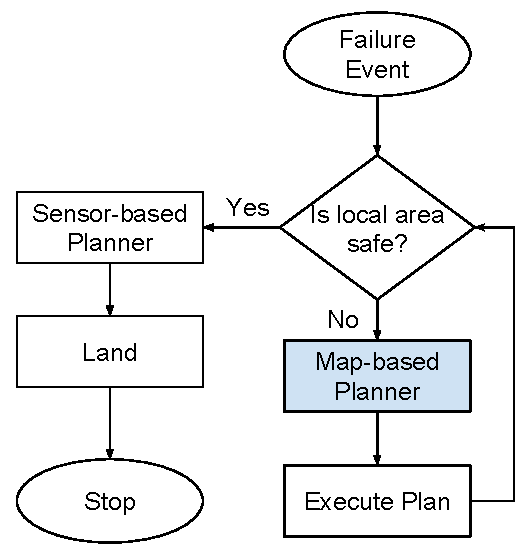
\includegraphics[scale=.65]{chapter_5_mapping/imgs/meta-level-planner.pdf}
\centering
\caption[Emergency planning logic.]{Emergency planning logic. Reprinted from Ref. \cite{ten_harmsel_emergency_2017}, originally published open access under a CC-BY 4.0 license. https://link.springer.com/article/10.1007/s10846-016-0370-z}
\label{fig:ch5_meta-level-planner}       % Give a unique label
\end{figure}


% \begin{figure}[ht!]
% \centering
% \includegraphics[width=.6\columnwidth]{icuas_metalevel_planner.pdf}
% \caption{Meta-level emergency planning architecture proposed in \cite{TenHarmsel2017}}
% \label{fig:ch5_meta-level-planner}
% \end{figure}

\subsection{Sensor Based Planning}\label{sec:ch5_local_sensor}
Onboard exteroceptive sensors including camera, radar, and LiDAR can provide a wealth of information about the surrounding environment for use in emergency landing planning. Ref. \cite{warren_enabling_2015} uses downward facing camera data to identify and characterize possible landing sites according to size, shape, slope, and nearby obstacles.
Ref. \cite{theodore_flight_2006} provides methods and experimental results of autonomous local landing using video and LiDAR data. Ref. \cite{desaraju_vision-based_2015} specifically identifies candidate landing sites on rooftops using a single camera, while Ref. \cite{forster_continuous_2015} identifies terrain-based landing sites in an image plane from 2D probabilistic elevation maps generated over terrain. In all cases landing site identification is only possible within the sensor field of view.

% Ref. \cite{goerzen2011minimal} presents a risk map for trajectory planning that translates risk to probability of an air vehicle reaching its destination, but this map is vehicle-centric whereas our risk map is environment-centric, e.g., mapping risk posed to an overflown community and population during an emergency.

\subsection{Map-Based Planning}\label{sec:ch5_map_based_planning}

There are two main approaches in generating landing sites for use in map-based \ac{UAS} emergency landing: one producing a specific landing site database and the other generating a risk grid from which landing sites can be selected. Both approaches, sometimes used together, rely on similar data sources such as census records, \ac{DSM} and map vector data but differ in output representations. A georeferenced database contains vector geometries of landing sites with associated meta data used for risk evaluation. A risk grid is a two or three dimensional data structure where each cell refers to the risk of a specific location on Earth.

Ref. \cite{di_donato_evaluating_2017} uses data such as census records, \ac{OSM}, and mobile phone records to quantify risk for unmanned aircraft requiring an emergency landing. Risk factors include risk to the vehicle, human population, property, and an area risk to assess the quality of a landing site. Landing sites such as open fields, grasslands, and highways are identified, risk evaluated, and stored in a landing site database. The proposed planning architecture uses this onboard database to select a risk-optimal landing site within a feasible flight footprint. After a landing site is chosen, path planning is performed at a constant altitude, assessing risk to people through a fusion of census data and mobile phone activity.

Ref. \cite{ten_harmsel_emergency_2017} proposes the use of three dimensional risk grids to identify landing sites and perform path planning for an energy-constrained multicopter in urban environments. A 3D occupancy grid to represent risk is generated as a combination of terrain, population, and obstacle costs.  Terrain risk is evaluated using slope as well as terrain type, census data is used to determine population risk, and property risk is assigned equally to all buildings. A linear combination of these risks is used to generate a final 3D grid for flight planning. In this grid a landing site is a \emph{terrain} cell that has a lower cost than a configurable threshold. All landing sites are treated equally, meaning the first landing site found by the planner is the ``optimal'' choice returned.

Ref. \cite{primatesta_ground_2020} proposes generation of a 2D risk map that quantifies  risk to population on the ground. The map is created taking into account an aircraft's model parameters and the local environment conditions while considering their uncertainties. The risk map is defined for a specific altitude and is the combination of several risk layers including population density, obstacles, sheltering, and no fly zones.

We propose an emergency landing framework that uses both a landing site database and a 3D risk grid to evaluate landing site risk and path risk as independent metrics. Our work is focused on Vertical Take-Off and Landing (VTOL) \ac{UAS} that might require an urgent landing but still have sufficient flight control to stably follow a prescribed path to touchdown. We provide a  multi-goal planner to trade off risk of landing sites with risk-optimal paths to each site while efficiently finding the minimum total risk solution. We uniquely identify usable area on flat rooftops using machine learning and computational geometry techniques. Previous efforts to quantify an \emph{area} risk of a landing site approximated risk as length or area of a site's buffered geometry \cite{di_donato_evaluating_2017}. However not all area in a landing site is suitable for landing. For example, many rooftops have obstacles such as air conditioning units, vents, and rooftop entrances. Additionally, the choice of a singular touchdown point at a chosen landing site is often simplified to be the centroid or pseudo-centroid of the site or cell \cite{di_donato_evaluating_2017, mejias_alvarez_forced_2009}. However both of these choices do not represent the optimal touchdown location with respect to ensuring flatness and distance from obstacles. We formulate the problem of choosing a touchdown position as finding the largest inscribed circle in its 2D polygon representation. Circle placement guarantees landing target coordinates are maximally separated from any obstacle or edge. 


% Selecting the landing zone point furthest from any obstacle is similar to the poles of inaccessibility (PIA) problem studied in \cite{garcia2007poles}. This problem requires finding the point within a 2D polygon that is furthest away from any border. Ref. \cite{polylabel} refines the work in \cite{garcia2007poles} to guarantee global optimality to a specified precision. Key contributions in \cite{polylabel} are the use of quadtrees to divide the search space and a heuristic that efficiently prunes non-optimal landing sites. Our definition of optimality inherits from this work and guarantees a selected flat landing zone is the furthest point away from any obstacle to a specified precision. Note that obstacles in landing zone are represented by holes/cutouts in the polygon and are accounted for. Our work effectively combines these techniques to identify flat landing zones to determine the optimal landing site location.


\subsection{Multi-Goal Planning}\label{sec:ch5_multi_goal_bg}

Multi-goal planning has two different  definitions:
\begin{enumerate}
    \item One start state and multiple goal states. The algorithm seeks to find the \emph{singular} goal/path pair that minimizes/maximizes an objective function.
    \item One start state, intermediary goal states, and a final end goal state. The algorithm seeks to find a connecting route, which includes \emph{multiple} connected state pairs, that minimizes/maximizes some objective function. This formulation is commonly called the travelling salesman problem (TSP) \cite{saha_planning_2003}.
\end{enumerate}
A visual representation of these definitions is shown in Figure \ref{fig:ch5_mg_example}. This chapter focuses on the first definition per Figure \ref{fig:ch5_mg_example}b.  Work by Ref. \cite{lim_uninformed_2014} investigated a form of multi-goal search using uninformed planners in a 2D grid. In this work all goals are valued equally with the objective to return paths for all start/goal combinations. Each start/goal pair can be treated as an independent path planning problem. Lim et al. propose reusing previous information, e.g.,  node expansions and costs, to reduce search overhead for the next goal. Results indicate that retaining information from previous searches reduces overhead in 2D grids when using uninformed search.

An objective or cost function may consider both the cost of a start/goal path and also the worth of the goal itself. Ref. \cite{sarne_multi-goal_2010} investigates efficient methods to conduct search for multiple agents seeking different products in a free market.  The authors propose a multi-goal planner that maximizes expected overall utility from the set of opportunities found (e.g., products/goals) minus the costs associated with finding that set. In this work the worth or value of a goal is probabilistic and can only be ascertained through search. The objective function aims to balance goal achievement reward against the cost of obtaining that goal.

In our work multiple landing sites (goals) will typically be identified. Risk is a function of path to each site as well as the site itself. Our objective is to find the singular goal/path pair which minimizes the combined risk of the landing site and a flight path from the initial \ac{UAS} location to that site. 
% Section \ref{sec:ch5_multi_goal_search_all} describes our proposed planner which finds the optimal landing site/path pair while minimizing the time to find it.
% Note that this process is conservative (i.e., the returned areas guarantee that minimum-area constraints are satisfied). However, it is not “optimal”. For example, one region might support several different circular landing areas, but only one will be returned by the algorithm. Moreover, candidate areas may have a larger simply connected region in a location different from the one returned.

\begin{figure}[ht!]
  \centering
  \begin{subfigure}[t]{0.25\linewidth}
    \centering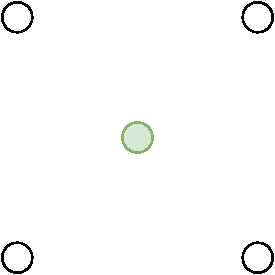
\includegraphics[width=.85\linewidth]{chapter_5_mapping/imgs/mg_all.pdf}
    \caption{\label{fig:ch5_mg_tsp_1} Case study with one initial state and four goal states.}
  \end{subfigure}
  \hfill
  \begin{subfigure}[t]{0.25\linewidth}
    \centering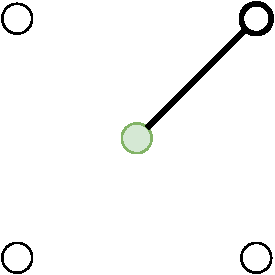
\includegraphics[width=.85\linewidth]{chapter_5_mapping/imgs/mg_sg_2.pdf}
    \caption{\label{fig:ch5_mg_sg_1} \protect\raggedright Planning to a \emph{single} goal despite multiple choices.}
  \end{subfigure}
  \hfill
  \begin{subfigure}[t]{0.25\linewidth}
    \centering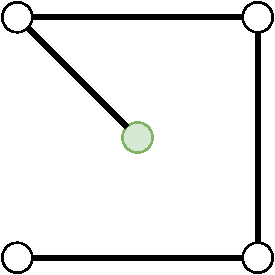
\includegraphics[width=.85\linewidth]{chapter_5_mapping/imgs/mg_tsp_2.pdf}
    \caption{\label{fig:ch5_mg_tsp_2} \protect\raggedright Traveling Salesman Problem with given initial state. }
  \end{subfigure}
%   \begin{subfigure}[b]{0.22\linewidth}
%     \centering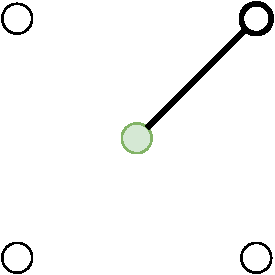
\includegraphics[width=\linewidth]{chapter_5_mapping/imgs/mg_sg_2.pdf}
%     \caption{\label{fig:ch5_mg_sg_2}}
%   \end{subfigure}%
  \caption[Comparison of multi-goal planning definitions]{Comparison of multi-goal planning definitions. The green state depicts the initial state, e.g., where the \ac{UAS} begins its emergency landing trajectory.  Unfilled circles are goal states.}
  \label{fig:ch5_mg_example}
\end{figure}


%\section{Preliminaries}\label{sec:ch5_problem}

\subsection{Urban Landscape and Rooftop Landings}

An emergency landing requires first identifying safe nearby landings sites.  Cities lack conventional emergency landing sites such as open fields or grasslands. Empty lots are often sparsely distributed, and parks may be unexpectedly occupied.  The satellite image in Fig. \ref{fig:ch5_challenge_urban} illustrates a typical urban landscape that affords rooftop landing. Obstacles on a flat rooftop, e.g., air conditioning units, can be removed from potential landing site surfaces. We identify rooftop landing sites given sufficient flatness and distance from obstacles and edges. 

\begin{figure}[ht]
    \centering
    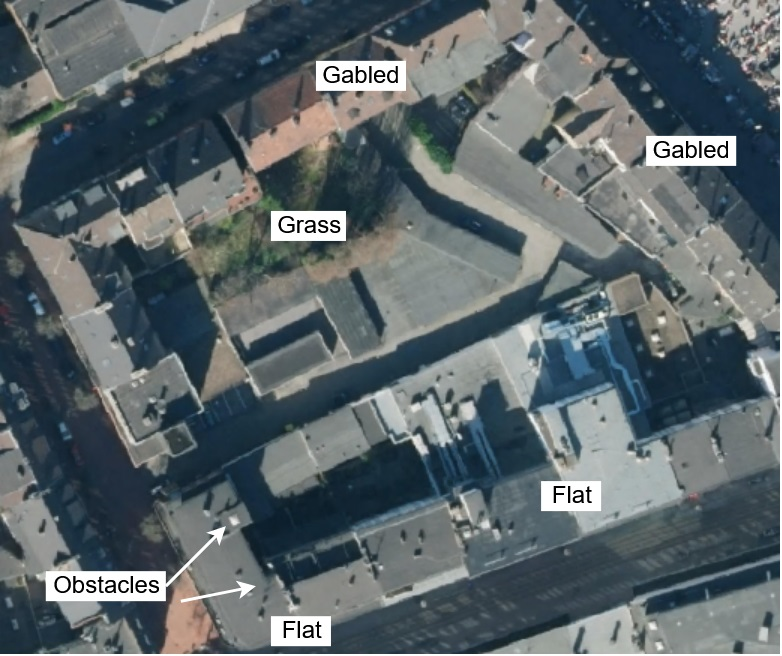
\includegraphics[clip, trim=0.0cm 0cm 0cm 0cm, width=0.45\linewidth]{chapter_5_mapping/imgs/challenge_urban-Page-2.jpg}
    \caption[Satellite image of an urban environment with multiple flat roof landing sites]{Satellite image of an urban environment with multiple flat roof landing sites. Select roof shapes and obstacles are labeled.}
    \label{fig:ch5_challenge_urban}
\end{figure}

Our proposed flight planner requires the vehicle to execute a stable approach to an emergency landing site.  Failure scenarios can be detected and handled in time to execute a controlled landing. Scenarios in which an urgent landing can be achieved without loss-of-control include: low battery energy, lost communication link, adverse weather, non-essential sensor or actuator failure, operator emergency landing directive, and non-cooperative aircraft nearby.  The methods and optimization techniques discussed in this chapter can be used for any VTOL aircraft. The case studies and simulations presented are specific to a multicopter in an urban environment.

% \subsection{Importing Open Street Map Data}
Steps required to construct a database of buildings and suitable ground-based landing zones (e.g., parks, fields, etc.) from  OpenStreetMap (OSM) are described in our previous work \cite{castagno_comprehensive_2018}.  This database is geospatial, in the sense that each row refers to a geographic entity (e.g., building or field) with polygonal shape. Meta data is also captured about each entity, e.g., height and land use. 

\section{Preliminaries}\label{sec:ch5_preliminaries}

\subsection{Coordinates and Landing Sites}

While map data will be globally georeferenced, low-altitude urban flights can be planned in a local Cartesian reference frame.
% On a global scale, a spherical coordinate system using latitude and longitude is often used; yet is not suitable for calculating \textit{planar} distance required in planning. Therefore a region specific \textit{projected} coordinate system is used such that distance and area are properly preserved. 
Let orthogonal bases for this Cartesian coordinate frame be denoted $\hat{\mathbf{e}}_x$, $\hat{\mathbf{e}}_y$, and $\hat{\mathbf{e}}_z$. The position of the \ac{UAS} body frame with respect to the local Cartesian reference frame can then be defined as:
\begin{equation}
\label{eq:ch5_position}
    {O}_{UAS}=x\,\hat{\mathbf{e}}_x+y\, \hat{\mathbf{e}}_y+z\, \hat{\mathbf{e}}_z = [x,y,z].
\end{equation}
A set of candidate landing sites are generated within a radial footprint $R$ defined as
\begin{align}
    \mathcal{S}_{ls} = \{ l_i, \ldots, l_n \}
\end{align}
where each $l_i$ refers to a landing site with properties
\begin{align}
    l_i = \{ \mathbf{c},\; r_{l}, \;r_{p} \} \\
    \mathbf{c} \in \mathbb{R}^3 \\
    r_{l}, r_{p} \in \mathbb{R}
\end{align}
where $\mathbf{c}$ is landing site location in the Cartesian reference frame, $r_{l}$ is landing site risk, and $r_{p}$ is path risk. Both risk values are in domain $[0,1]$. Landing site risk is calculated offline and represents the risk intrinsic to touching down at that landing site. Path risk must be calculated online and accounts for the path distance and proximity to obstacles. The calculation of $r_{l}$ is shown in Section \ref{sec:ch5_risk_model}, while $r_{p}$ is described in Section \ref{sec:ch5_cost_maps}.

\subsection{3D Path Planning with Mapped Obstacles}\label{sec:ch5_path_planning}

Path planning requires a cost function to guide search space exploration in pursuit of a feasible and optimal solution. For discrete search planners, the space must first be discretized into a graph ${G}({V},{E})$, where ${V}$ denotes graph vertices with edge set ${E}$ and associated transition costs. This graph is defined implicitly for a 3D grid. The vertices are the cells/voxels accessed with indices $(i,j,k)$. The edge of each cell are dynamically computed from the 26 neighbors. In a mapped environment, A* search applies a heuristic to reduce search overhead.  A* sums actual path cost $g(n)$ and heuristic $h(n)$ estimating cost-to-go to form node $n$ total cost $f(n)$:
\begin{align}
    c(n', n) &= \text{dist}(n', n) 
    \cdot (1 + \text{risk}(n)) \label{eq:ch5_risk_function_planner} \\ 
    g(n) &= g(n') + c(n', n)\\
    f(n) &= g(n) + h(n)
\end{align}
%    h(n) &= \text{dist}(n, goal)
where $c$ is transition cost from previous node $n'$ to current node $n$, 
% $g$ is cumulative cost, $h$ is heuristic cost, and $f$ is estimated total cost, defined above
$\mathbf{dist}(\cdot)$ is Euclidean distance between adjacent nodes $n'$ and $n$, and $\mathbf{risk}(\cdot)$ represents normalized risk encoded in the 3D map. 
%The path risk, $r_p$, is the total accrued cost of the path to reach the goal node normalized by $R$.
The search space is limited to cells within the the radial footprint $R$ to bound worst case scenarios. We use a 3D octile distance heuristic $h(n)$ which has been shown much more effective than Euclidean distance \cite{nash_lazy_2010}.  %The octile distance heuristic efficiently guides the planner to a goal state especially where straight line paths are possible (e.g., flying above rooftops).
% The planner traded off between paths resulting in high risk to the aircraft (e.g., flying close to nearby buildings) and the distance of travel required.  The multidimensional risk map defined above, $R_{map}$, is used by our A* path planner to generate optimal collision free paths from the current \ac{UAS} position to a landing site. 


%We refer the reader to our previous paper to construct this database as it will be assumed to be created for subsequent processing.

\begin{figure}[!t]
    \centering
    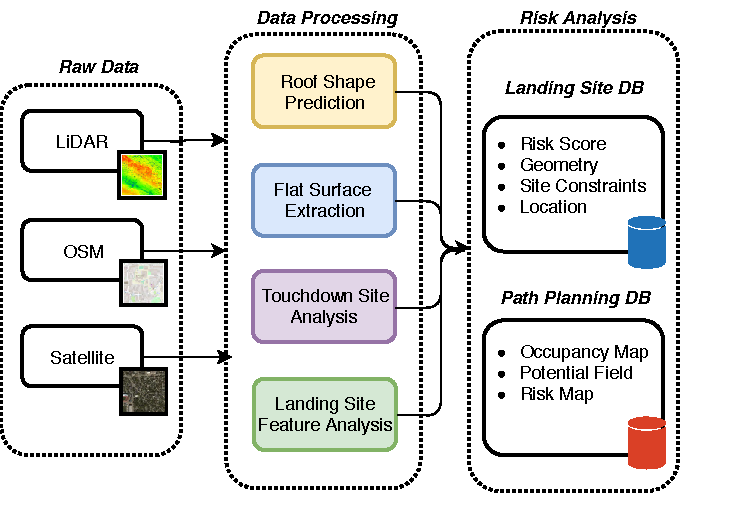
\includegraphics[clip, trim=0.0cm 0cm 0cm 0cm, width=0.7\linewidth]{chapter_5_mapping/imgs/data_preprocessing-Page-1.pdf}
    \caption[Processing pipeline to construct landing site and occupancy map databases]{Processing pipeline to construct landing site and occupancy map databases. Landing sites and occupancy map are risk evaluated.}
    \label{fig:ch5_overview_processing}
\end{figure}

\section{Landing Site Database}\label{sec:ch5_landing_site_database}

 Data is fused from OSM, LiDAR, and satellite image sources to construct a feature-rich landing site database. Figure \ref{fig:ch5_overview_processing} provides an overview of the data processing pipeline that provides the features needed to construct a landing site database with risk metrics and maps.
% Our previous paper \cite{Castagno2018ICUAS} outlines procedures for extracting data from \ac{OSM}to construct a geospatial database that describes landing sites as simple polygons with labelled attributes, e.g. landuse and height. 
Below, Section \ref{sec:ch5_flat_like} summarizes the machine learning (ML) process detailed in \cite{castagno_comprehensive_2018} to identify flat-like rooftops from which landing sites are identified. Section \ref{sec:ch5_usable_area} describes our procedure to refine each landing site by determining usable area. Section \ref{sec:ch5_method_circle} describes a method to compute the touchdown location on large flat surfaces. Landing site risk models are described in Section \ref{sec:ch5_risk_model}.

\subsection{Flat-like Roof Identification}\label{sec:ch5_flat_like}
%  Chapter  authors have previously published data and ML models for predicting roof shape by fusing building outlines, satellite images, and airborne LiDAR data \cite{castagno_roof_2018}.
Information on building roof shape is sparse in existing  databases. Chapter 4 shows that a total accuracy of 86\% is achievable when evaluating a trained ML pipeline on independent test sets. By adjusting the confidence threshold to 50\%, precision and recall of 95\% and 75\% can be achieved in classifying flat-like roofs in cities.  This chapter employs the roof shape prediction model from Chapter 4 to label building roof shapes for subsequent landing site identification. High precision is necessary to assure that few false positives will be identified. Note that offline map building allows  human inspection of city-wide rooftop landing sites to assure each identified unsafe site is pruned prior to landing site database use by a UAS.

\begin{figure}[!ht]
 \centering
\begin{subfigure}[b]{0.33\linewidth}
\centering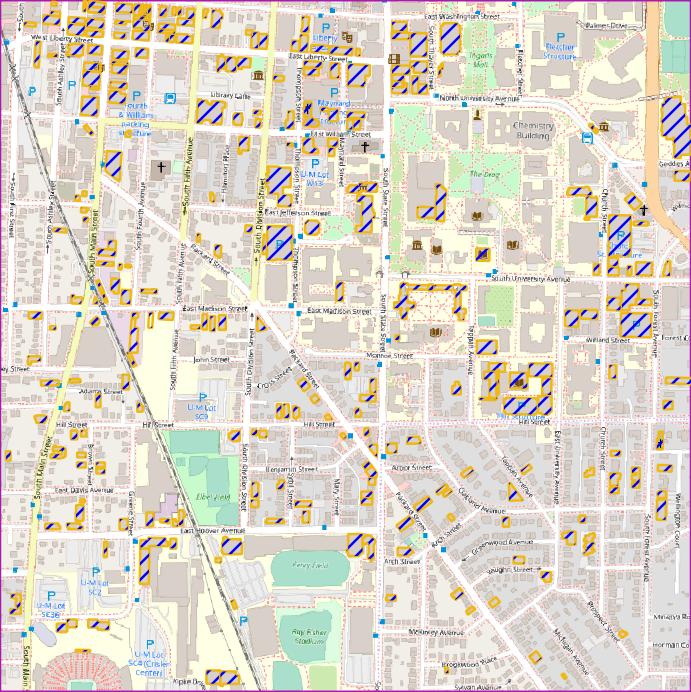
\includegraphics[clip, trim=0.0cm 0.0cm 0.0cm 0.0cm, width=\linewidth]{chapter_5_mapping/imgs/aa-flat-buildings-map.png}
 \caption{Ann Arbor, Michigan}\label{fig:ch5_aa-flat}
\end{subfigure}
\begin{subfigure}[b]{0.33\linewidth}
\centering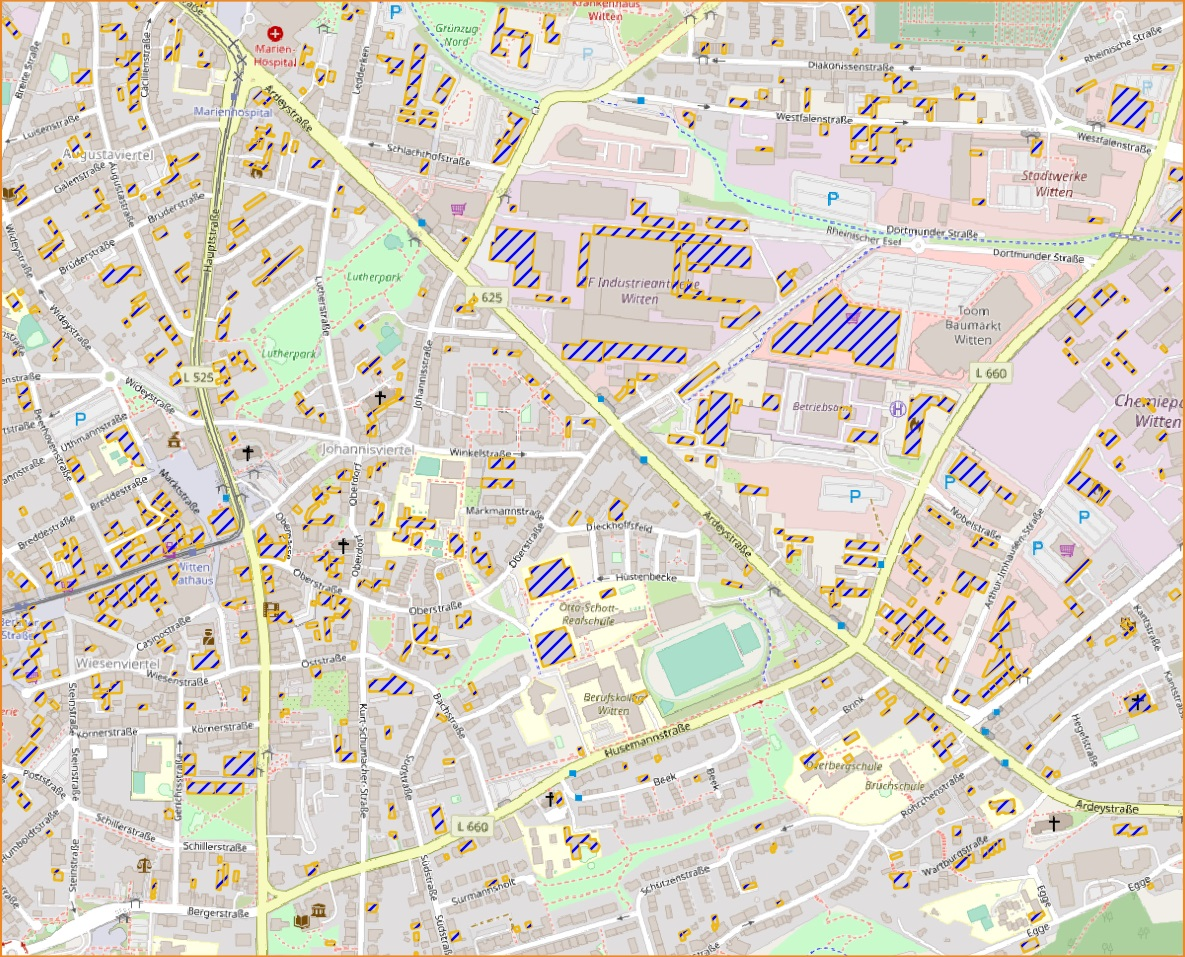
\includegraphics[clip, trim=0.0cm 0.0cm 0.0cm 0.0cm, width=\linewidth,height=110pt]{chapter_5_mapping/imgs/witten-flat-buildings-map.jpg}
 \caption{Witten, Germany}\label{fig:ch5_wt-flat}
\end{subfigure}
 \begin{subfigure}[b]{0.30\textwidth}
 \centering
 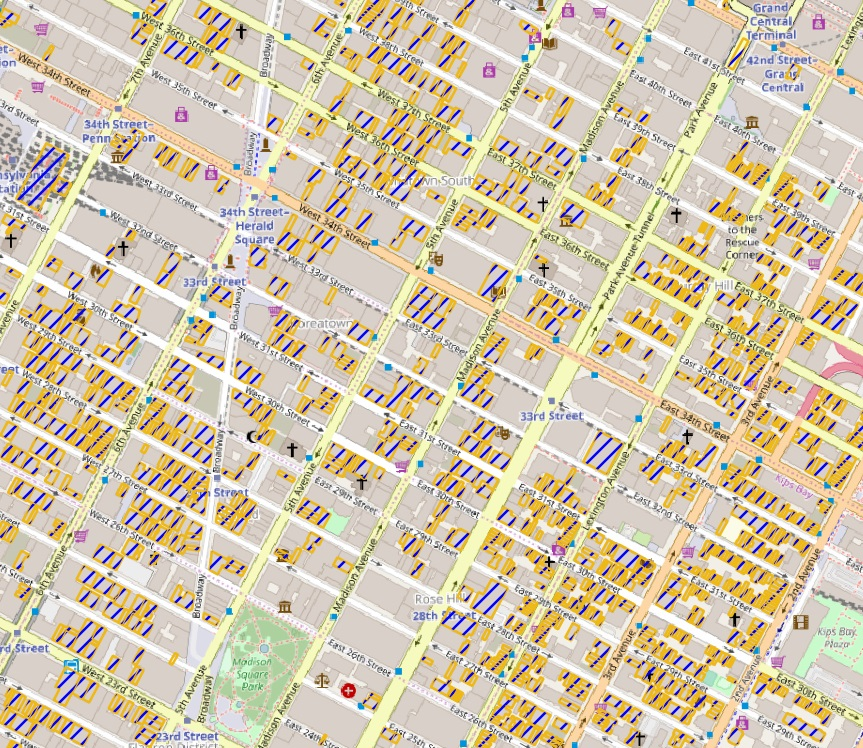
\includegraphics[clip, trim=0.0cm 0.0cm 0.0cm 0.0cm, width=\linewidth,height=110pt]{chapter_5_mapping/imgs/ny-flat-buildings-map.jpg}
%   \rule{\linewidth}{\dimexpr 2\linewidth+2\baselineskip+6pt}
   \caption{Manhattan, New York}\label{fig:ch5_ny-flat}
 \end{subfigure}
%   \sidecaption[t]
 \caption[Maps of predicted flat rooftops in three cities.]{Maps of predicted flat rooftops in three cities. Buildings with a predicted flat-like roof shape are outlined in dark yellow with blue dashed lines through the center.  Parks and grasslands are shown in green. Maps from \copyright OpenStreetMap contributors and \copyright CARTO. License: Open Database License: https://www.openstreetmap.org/copyright}\label{fig:ch5_all_flat_buildings}
\end{figure}

Figure \ref{fig:ch5_all_flat_buildings} shows results of our roof prediction model for the cities of Ann Arbor, Michigan, Witten, Germany, and mid-town Manhattan in New York City. In previous work only parks and grasslands were processed to identify emergency landing zones. This work adds new landing site options identified from the illustrated flat-like rooftops as described below. 
%in Section \ref{sec:ch5_usable_area}. 

% \subsection{Identifying Safe Touchdown Sites}

%  Section \ref{sec:ch5_methods_plane_extaction} outlines our proposed methods of identifying \emph{usable} landing site area for ground and rooftops described as non-convex 2D polygons. Section \ref{sec:ch5_method_circle} describes our proposed to find \emph{optimal} touchdown landing sites in said polygons.

% Previous work for UAV emergency landing only uses landing site meta data (e.g. land use, census data) and total area as metrics for determining landing site risk \cite{Castagno2018ICUAS}. However not all area in a landing site is suitable for landing; for example many rooftops have obstacles such as ac-units, superstructures, and rooftop entrances. In addition the choice of a singular touchdown point on a chosen landing site area is often simplified to be the centroid or psudo-centroid of the site \cite{di2017evaluating}. However both of these choices do not represent the optimal touchdown location in respect to ensuring flatness and distance from obstacles. We formulate the problem of choosing an optimal touchdown position on a 2D polygon as finding the largest inscribed circle in a 2D polygon. The circle placement guarantees optimal position on a landing site furthest from any obstacle or edge. 

% The following section presents a process of identifying flat surfaces on buldings from airborne LiDAR data, and subsequintely identified large circular 

\begin{figure}[t]
  \centering
  \begin{subfigure}[b]{0.45\linewidth}
    \centering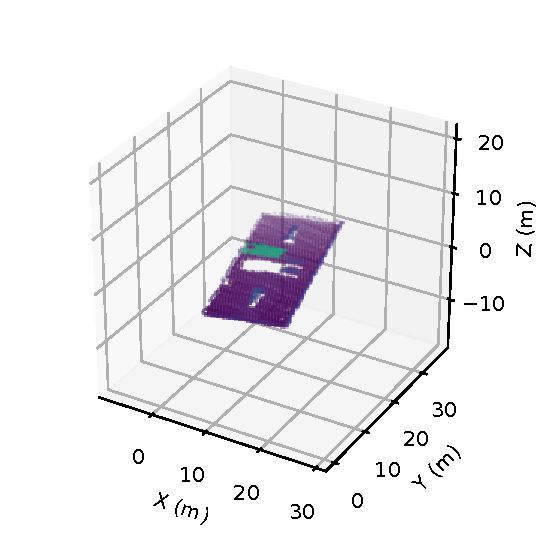
\includegraphics[clip, trim=1.6cm 0.2cm 0.1cm 0.5cm, width=125pt]{chapter_5_mapping/imgs/74200284_points.pdf}
    \caption{\label{fig:ch5_pc_example}}
  \end{subfigure}
  \begin{subfigure}[b]{0.45\linewidth}
    \centering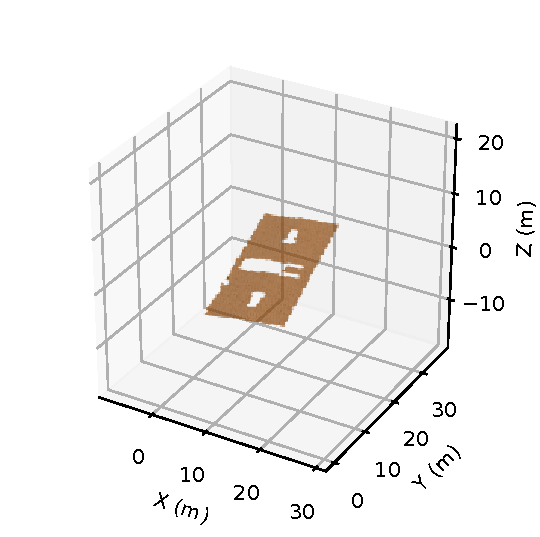
\includegraphics[clip, trim=1.6cm 0.2cm 0.1cm 0.5cm, width=125pt]{chapter_5_mapping/imgs/74200284_trimesh.pdf}
    \caption{\label{fig:ch5_trimesh_example}}
  \end{subfigure}
  \begin{subfigure}[b]{0.45\linewidth}
    \centering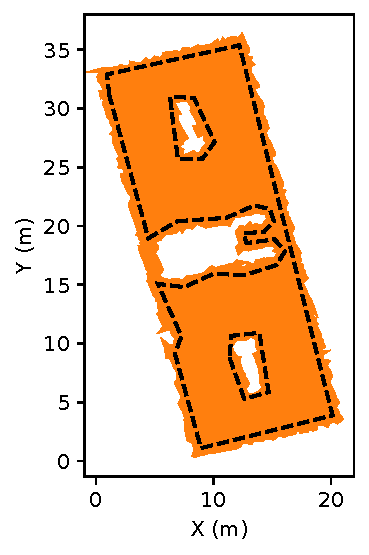
\includegraphics[width=100pt,height=125pt]{chapter_5_mapping/imgs/74200284_polygonbuffer.pdf}
    \caption{\label{fig:ch5_polygon_example}}
  \end{subfigure}
  \begin{subfigure}[b]{0.5\linewidth}
    \centering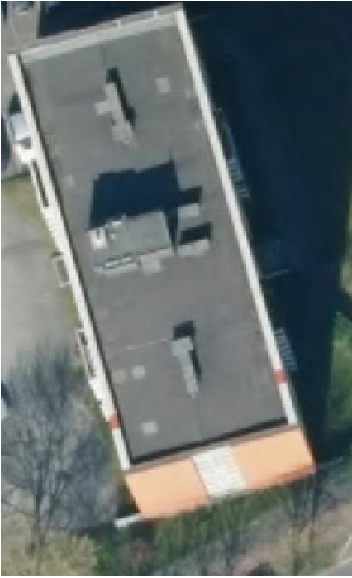
\includegraphics[width=75pt,height=125pt]{chapter_5_mapping/imgs/74200284_satellite_simple.pdf}
    \caption{\label{fig:ch5_satellite_example}}
  \end{subfigure}%
  \caption[Flat surface extraction from rooftops]{Flat surface extraction from rooftops. Point cloud data for a building is displayed in (\subref{fig:ch5_pc_example}); (\subref{fig:ch5_trimesh_example}) shows the generated planar triangular mesh.  Conversion of the 3D mesh to a 2D polygon is shown in (\subref{fig:ch5_polygon_example}) with subsequent polygon inward buffering and simplification shown in dashed lines.  A reference satellite image is shown in (\subref{fig:ch5_satellite_example}).}
  \label{fig:ch5_example_usable}
\end{figure}

\subsection{Flat Surface Extraction for Usable Landing Area}\label{sec:ch5_usable_area}

%Usable landing area is defined as a flat-like surface free of any obstacles. 
Airborne LiDAR point cloud data is used to determine planarity, shape, and extent of potential \ac{UAS} landing site surfaces.  %Polygon outlines are constructed of proposed landing sites. 
Proposed polygonal landing sites are buildings with predicted flat-like roof shapes and terrain locations with land use keywords listed in Table \ref{table:ch5_terrain_property_costs}.  A point-in-polygon ray casting algorithm is used to generate the point set $P_{ls}$ \cite{samosky_sectionviewsystem_1993} where point clouds only reside in the outline of the landing site. 

Next, flat surface extraction from $P_{ls}$ is performed using the Polylidar3D algorithm developed by the authors in \cite{castagno_polylidar3d_2020}. The algorithm works by generating triangular meshes of an input point cloud, filtering triangles by planarity and edge length, extracting subsets of the mesh which are spatially connected, and finally converting the mesh to a polygon format. Polylidar3D is configurable by user provided planarity constraints and maximum triangle edge length. This guarantees the polygon can represent flat surfaces with interior holes denoting obstacles. Highlights of this procedure are shown in Figure \ref{fig:ch5_example_usable}. 

After the flat region is extracted, e.g., the orange polygon in Figure \ref{fig:ch5_example_usable}c, this polygon is buffered inward and simplified as denoted by dashed lines. The buffering process is defined as the Minkowski difference of the polygon with a circle with radius equal to a buffer distance \cite{agarwal2002polygon}. We set the buffer distance to 0.5 meters which contracts the exterior hull and expands the interior holes.  Afterwards we use the Douglas-Peucker's simplification algorithm to remove redundant vertices and ``smooth'' the polygon \cite{douglas_algorithms_1973}.
% Both the simplification and buffering process is performed by the GEOS library.
Narrow flat surfaces can be removed in this process as shown near the (6, 17) point in subfigure (c). The final output of this procedure is a set of polygons denoting flat and obstacle free surfaces.

\subsection{Touchdown Points}\label{sec:ch5_method_circle}\label{sec:ch5_touchdown}
Once flat surface(s) have been extracted from potential rooftop and ground-based landing sites and represented as polygons, an ideal landing \emph{touchdown point} must be defined. We define this ideal point to be farthest from any non-flat region or obstacle. In other words, the touchdown point is the furthest distance away from the exterior hull and any interior holes. This requirement may be framed as the Poles of Inaccessibility problem \cite{garcia-castellanos_poles_2007} and the Polylabel algorithm as proposed in \cite{noauthor_github_2018-3} provides a solution. This algorithm aims at efficiently determining the largest inscribed circle in a polygon within a prescribed tolerance. The largest inscribed circle for the same rooftop in Figure \ref{fig:ch5_example_usable} is shown in Figure \ref{fig:ch5_touchdown_zones}a. 
There are additional suitable touchdown sites on this rooftop that can be used. We propose Algorithm \ref{alg:ch5_touchdown_extraction} to capture the remaining touchdown points as a ranked list of circles. The algorithm begins by calling Polylabel to find the point and radius representing the largest circle inside an input polygon $P$.  A 16-sided polygon representation of this circle is created denoted $P_c$. If the radius is below a user provided minimum radius $r_{min}$ then the empty set is returned. $P_c$ is subtracted from the input polygon to create a smaller polygon $P_{diff}$. The procedure ends by returning the union of $P_c$ and the result of a recursive call to \texttt{TouchdownExtraction} with $P_{diff}$ as the input polygon. This recursive call continues the process of finding next largest circle. The end result is an ordered set of circular polygons with a radius greater than $r_{min}$. This minimal radius is user defined and should determined by \ac{UAS} characteristics. Visualization after the first and second procedure call are in Figure \ref{fig:ch5_touchdown_zones}a,b respectively, with the final rankings shown in Figure \ref{fig:ch5_touchdown_zones}c.

\begin{figure}[ht]
  \centering
  \begin{subfigure}[b]{0.32\linewidth}
    \centering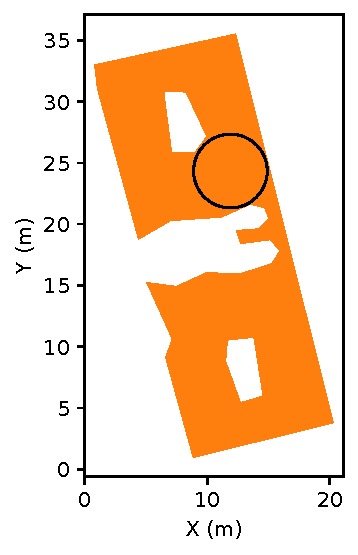
\includegraphics[width=80pt,height=125pt]{chapter_5_mapping/imgs/74200284_polygonbuffer_lc.pdf}
    \caption{\label{fig:ch5_polylabel_example}}
  \end{subfigure}
  \begin{subfigure}[b]{0.32\linewidth}
    \centering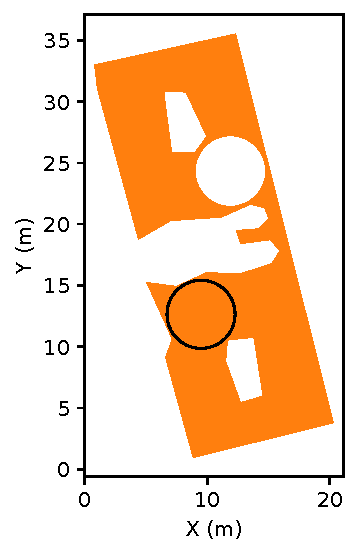
\includegraphics[width=80pt,height=125pt]{chapter_5_mapping/imgs/74200284_polygonbuffer_second_lc.pdf}
    \caption{\label{fig:ch5_polylabel_example_second}}
  \end{subfigure}%
  \begin{subfigure}[b]{0.32\linewidth}
    \centering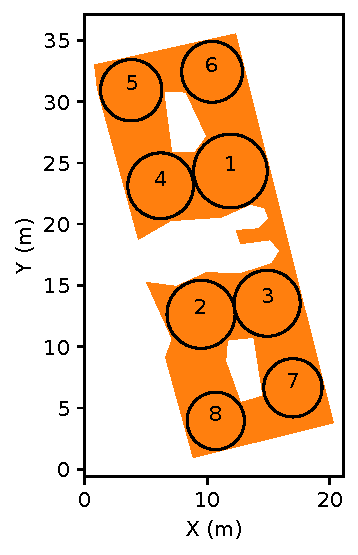
\includegraphics[width=80pt,height=125pt]{chapter_5_mapping/imgs/74200284_polygonbuffer_all_lc.pdf}
    \caption{\label{fig:ch5_polylabel_example_all}}
  \end{subfigure}%
  \caption[Touchdown point extraction on rooftops]{Touchdown point extraction on rooftops. Rooftop surface shown in orange. The best (largest circle) landing zone is shown in (\subref{fig:ch5_polylabel_example}). (b) Polygon subtraction of a previously found touchdown zone. The complete ranked touchdown site set is shown in (\subref{fig:ch5_polylabel_example_all}).}
  \label{fig:ch5_touchdown_zones}
\end{figure}

\begin{algorithm}
    \SetKwInOut{Input}{Input\hspace{0.3cm}}
    \SetKwInOut{Output}{Output}
    \SetStartEndCondition{ }{}{}%
    \SetKwProg{Fn}{def}{\string:}{}
    \SetKwFunction{Range}{range}%%
    \SetKw{KwTo}{in}\SetKwFor{For}{for}{\string:}{}%
    \SetKwIF{If}{ElseIf}{Else}{if}{:}{elif}{else:}{}%
    \SetKwFor{While}{while}{:}{fintq}%
    % \AlgoDontDisplayBlockMarkers\SetAlgoNoEnd\SetAlgoNoLine%

    \Input{\hspace{0.2cm}Polygon: $P$, Mininum Radius: $r_{min}$}
    \Output{\hspace{0.2cm}Set of Polgyon Circles}
    
    % $\mathcal{S}_P = \{ P\}$ \\
    $point, r = \operatorname{Polylabel}(P)$ \\
    $P_{c} = \operatorname{PolgyonCircle}(point, r)$ \\
    \uIf{$r < r_{min}$}{
        return $\emptyset$
    }
    $P_{diff}$ = $P - P_{c}$ \\
    return $P_{c} \cup \operatorname{TouchdownExtraction}(P_{diff}, r_{min})$
    \caption[Touchdown Point Extraction]{TouchdownExtraction}
    \label{alg:ch5_touchdown_extraction}
\end{algorithm}

The final landing site chosen for each surface is the top ranked touchdown site. The remaining circles are kept in the database for further use in risk assessment.

\subsection{Landing Site Risk Model}\label{sec:ch5_risk_model}

Each landing site corresponds to the largest clear touchdown area on either flat terrain or building rooftop surfaces. This chapter adopts the risk model first presented in Ref. \cite{castagno_comprehensive_2018}.  Risk is quantified as vehicle cost ($C_v$), property cost ($C_p$), and human occupancy cost ($C_o$). Each of these risks are numeric values created from a functional composition of the attributes of each feature (land use, available area, etc.) as outlined in Sections \ref{sec:ch5_vehicle_cost}, \ref{sec:ch5_property_cost}, and \ref{sec:ch5_occupancy_cost} respectively. Landing site risk is the weighted sum
\begin{align}\label{eq:ch5_landing_site_risk}
    r_l = w_v \cdot C_v + w_s \cdot C_p + w_o \cdot C_o \\
    w_v + w_s + w_o = 1 \notag
\end{align}
where $w_v, w_s,$ and $w_o$ are weights for vehicle, property and human occupancy cost respectively.

\subsubsection{Vehicle Cost}\label{sec:ch5_vehicle_cost}

We denote risk to the \ac{UAS} "vehicle" as
\begin{align}
    C_v = w_t C_t + w_{a}C_{a} + w_{ca} C_{ca}\\
    C_v,\; C_t,\; C_a,\; C_{ca} \in [0,1]
\end{align}
where $C_t$, $C_a$, and $C_{ca}$ are risk-based costs associated with terrain type, usable area, and cumulative usable area respectively.  The variables $w_t$, $w_a$, and $w_{ca}$ are the user-defined weights aggregating these metrics into a total $C_v$ value.

\subsubsection{Terrain Cost}

Terrain cost $C_t$ approximates the risk posed to the vehicle due to landing on a specific type of terrain. We use keywords gathered from \ac{OSM} that describe type of terrain. Following a similar taxonomy from \cite{di_donato_evaluating_2017}, these  keywords are aggregated into groups and assigned costs as shown in Table \ref{table:ch5_terrain_property_costs}.  The trend of these costs is that groups with generally unoccupied open areas, such as Group 2, have lower risk than groups with possible cluttered areas, such as Group 5. Building rooftops, Group 1, have a slightly higher terrain cost than Group 2 because of increased risk at landing at higher altitudes. Group 7, industrial and commercial areas, have more diverse and uncertain terrain characteristics and assigned a higher cost. These costs are subjective in nature thus would be refined later by stakeholders.

\begin{table}[!ht]
\centering
\caption{Terrain Type and Property Cost}
\label{table:ch5_terrain_property_costs}
\begin{tabular}{p{1.5cm}p{4.7cm}p{1.6cm}p{1.7cm}}
\hline\noalign{\smallskip}
Group   & Keywords & Terrain ($C_t$) & Property ($C_p$) \\ % & Description     
\noalign{\smallskip}\hline\noalign{\smallskip}
Group 1 & \begin{tabular}[t]{@{}l@{}}building rooftops \end{tabular}                               & 0.25 & 0.5 \\
Group 2 & \begin{tabular}[t]{@{}l@{}}brownfield, grass, grassland\\ village green, greenfield\end{tabular}                               & 0.0 & 0.0  \\ %  & \begin{tabular}[t]{@{}l@{}}Land with smooth surface\\ and generally obstacle free\end{tabular}                 \\
Group 3 & \begin{tabular}[t]{@{}l@{}}meadow, cemetery, scrub\end{tabular}                                             & 0.25 & 0.0 \\ % & \begin{tabular}[t]{@{}l@{}}Land with semi-smooth surface \\  and generally obstacle free\end{tabular}           \\
Group 4 & water, riverbank                                                                                & 0.75 & 0.0  \\ % & \begin{tabular}[t]{@{}l@{}}Land unfit for landing\\ but obstacle free\end{tabular}                             \\
Group 5 & \begin{tabular}[t]{@{}l@{}}recreation ground, garden, \\ golf course, track, pitch, \\ playground, common, park\end{tabular} & 0.5 & 0.25  \\%  & \begin{tabular}[t]{@{}l@{}}Land with smooth surface\\ but with possibilities\\ of obstacle\end{tabular}        \\
Group 6 & parking                                                                                                                        & 0.75 & 0.75 \\ % & \begin{tabular}[t]{@{}l@{}}Land with semi-smooth \\ surface but with \\ possibilities of obstacle\end{tabular} \\
Group 7 & industrial, commercial                                                                                                         & 1.0 & 1.0 \\ %  & \begin{tabular}[t]{@{}l@{}}Land with unknown \\ terrain type and obstacle\end{tabular}                         \\ \bottomrule
\end{tabular}
\end{table}

\subsubsection{Area Cost}
Large flat surfaces pose less risk to \ac{UAS} than small clearings. Our proposed risk model quantifies this as an area cost $C_a$. We propose Eq. \ref{eq:ch5_area_cost} to map small areas to high risk (1), average areas to medium risk (0.5), and large areas to low risk (0). This piecewise exponentially decaying function is governed by user-defined minimum area $A_{min}$ and maximum area $A_{avg}$.  Note that $A_{min}$ is the area of the circle with radius $r_{min}$ used in Algorithm \ref{alg:ch5_touchdown_extraction}. These values would take UAS-specific landing area requirements into account.
\begin{align}\label{eq:ch5_area_cost}
    \operatorname{Area\; Cost} (a) = \begin{cases} 
       1 & a \leq A_{min} \\
       e^{-c \cdot a} &  a > A_{min}
    %   e^{-c \cdot (a - A_{min})} &  a > A_{min}
   \end{cases} \\
   c = \frac{\ln{2}}{A_{avg}- A_{min}}
\end{align}
An example of this mapping is shown in Figure \ref{fig:ch5_ny_area_cost}.

\begin{figure}[ht]
    \centering
    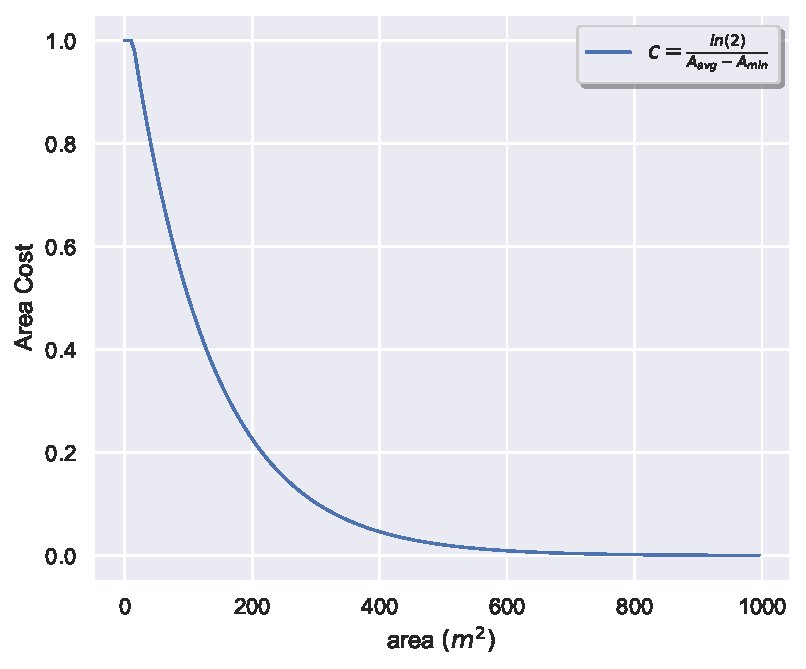
\includegraphics[clip, trim=0.2cm 0cm 0cm 0cm, width=0.5\linewidth]{chapter_5_mapping/imgs/area_cost.pdf}
    \caption[Mapping area size to risk]{Mapping area size to risk. Function maps area size to a cost value between [0, 1]. In this example $A_{avg}$ and $A_{min}$ are 100 and 12.5$m^2$, respectively. }
    \label{fig:ch5_ny_area_cost}
\end{figure}


\subsubsection{Cumulative Area Cost}
A landing site that is nearby additional sites has advantage to landing sites with no other nearby options. 
% It is possible that a landing site from the database does not have the actual low risk qualities desirable at the time of landing.  
We capture this metric as a cumulative area cost $C_{ca}$.  The cumulative area of all touchdown sites available on an individual building or terrain surface is computed as shown in Figure \ref{fig:ch5_touchdown_zones}c.  This area is then mapped to $C_{ca}$ using equation \ref{eq:ch5_area_cost}.

\subsubsection{Property Cost}\label{sec:ch5_property_cost}
\ac{UAS} may inadvertently damage a landing site in the event of an unplanned landing. Landing site characteristics can impact the likelihood, severity, and cost of damage. Table \ref{table:ch5_terrain_property_costs} provides example normalized estimates for the costs of similar landing sites. The proposed metric assigns increase cost to areas that may be damaged in the event of a high impact crash. Natural terrain areas have low cost while buildings and other maintained properties have higher cost. Parking lots and industrial areas are marked with the highest cost to people and property, e.g., cars, pedestrians. %Key stakeholders should later refine such estimates or construct detailed risk models.

\subsubsection{Human Occupancy Risk Mapping}\label{sec:ch5_occupancy_cost}

Overflight risk to people is typically estimated with an occupancy grid based on Census records \cite{stevenson_estimated_2015-1, ten_harmsel_emergency_2017, ancel_real-time_2017}.  Census records in the United States are released every 10 years in an aggregated form in which the smallest areal unit is the census block. The size of a census block may vary from a city block to a much larger area in a rural community. For example in New York City the average size of a census block is a 121X121 meter square but with substantial variance over the city landscape.  This average resolution is suitable for city-wide risk assessment but not ideal for higher-resolution occupancy mapping. Techniques such as daysymetric modelling \cite{nagle_dasymetric_2014-1} are used to improve the spatial resolution of Census datasets at the cost of greater uncertainty \cite{dmowska_high_2017-1}.

Census records only provide information of where people reside which is most often representative of a region's nighttime population \cite{di_donato_evaluating_2017}.  \ac{UAS} will fly at all times of the day so time-varying population estimates are critical for accurate risk assessment. Work by Ref \cite{di_donato_evaluating_2017} fused census data with  publicly available mobile phone call detail records (CDR) in Italy to generate a temporal population model for \ac{UAS} risk assessment. Results indicated significant population migration throughout the day reinforcing the inadequacy of using a static population model. However, CDRs are not generally open for public use, and access to other real-time data streams such as aggregated mobile phone GPS is limited. Most of the landing sites proposed in this chapter are on flat rooftops likely to be unoccupied despite high building occupancy. Many population risk models introduce a shelter factor which estimates zero casualties whenever the building is not penetrated, e.g., during a \ac{UAS} rooftop landing \cite{melnyk_third-party_2014-1}.

This work requires risk assessment for landings sites and paths over small radial footprints ($<250$ m). The authors have previously used census data to assess population risk in this situation. However, a static low-resolution population model may provide misleading risk assessments. Therefore this work does not use population risk metrics by setting $w_o$ to 0 in Eq. \ref{eq:ch5_landing_site_risk}. Our combined risk model will include path length, which when minimized, is a proxy to minimizing the risk to people during urgent landings so long as population is uniformly distributed rather than clustered, e.g., for special events not modeled in census data.

% Census records to assess population density to help quantify $C_p$. However the authors now believe that this data source to be inappropriate in assessing risk in urban city centers. Census data only provides semi-accurate population estimates at night time and often at resolution sizes to large to be usable to delineate landing sites in small emergency footprints. City populations are not static and change rapidly throughout business work hours. A better data source and model is needed which accurately accounts for the liveliness of a city at finer resolutions ($30m^2$). Mobile phone call detail records, city transportation metrics, and mobile phone GPS are all excellent data sources to construct such a model. Unfortunately almost none of these data are public or are specific to one city. For these reasons $C_p$ was set to 0.

% Distance metric is more valuable in describing population risk. Cite perdros paper, equations and papers. Talk about shelter costs.


\section{Three-Dimensional Maps for Path Planning}\label{sec:ch5_cost_maps}\label{sec:ch5_occupancy_map}


% \subsection{Obstacle Occupancy and Risk Mapping}\label{sec:ch5_occupancy_map}

Let the city occupancy and risk map generated for path planning be denoted $R_{map}$. This map is a dense 3D voxel structure of size $M\times N \times K$, where the rows, columns and slices are $M, N$ and $K$ respectively. Each cell is indexed by triplet $(i, j, k)$  returning occupancy and risk information for a specific position. Publicly available airborne point cloud data or digital surface maps (DSM) may be used as the primary data source to construct $R_{map}$. A DSM is a raster where each pixel holds a height value above Earth's Mean Sea Level (MSL) including buildings and foliage. Such data sources are often georeferenced in a projected coordinate system which minimizes distortion of shape, area, or distance. This Cartesian coordinate system is ideal for path planning thus is carried into the voxel map. The rest of this procedure assumes the use of a DSM with equal pixel resolution and associated affine transformation matrix to convert from pixel space to the local Cartesian frame.

The procedure begins with a city DSM of size $M\times N$. The minimum and maximum height, $z_{min}$ and $z_{max}$, are computed from the DSM. The value of $z_{max}$ is bounded at 400 feet above local terrain level in this work. Note that FAA Part 107 restricts flying small \ac{UAS} more than 400 feet above the tallest nearby obstacle \cite{federal_aviation_administration_code_2016}. An affine transformation matrix $A$ is generated for $R_{map}$:
% please double check weather I am interpreting this FAA rule correctly
\begin{align}
        A = \begin{bmatrix} \label{eq:ch5_affine_matrix}
        x_{res} & 0 & 0 & x_{min} \\
        0 &  -y_{res} & 0 & {y_{max}} \\
        0 &  0 & z_{res} & {z_{min}} \\
        \end{bmatrix}  \\
        \begin{bmatrix}x & y & z  \end{bmatrix}^T = A \cdot \begin{bmatrix}i & j & k  \end{bmatrix}^T \label{eq:ch5_affine_equation}
\end{align}
where $x_{min}$, $x_{res}$, $y_{max}$, and $y_{res}$ are provided by the DSM affine matrix. Eq. \ref{eq:ch5_affine_equation} performs the conversion from 3D voxel space to the local Caretesian coordinate system.  
% The values of $x_{res}$, $y_{res}$, and $z_{res}$ are all equal and will set to 2 meter/pixel. 
The number of slices, K, is equal to $\floor*{\frac{z_{max} - z_{min}}{z_{res}}}$. An $M \times N \times K$ data structure storing unsigned 8 bit integers is zero initialized to represent $R_{map}$.

The occupancy map is generated similar to \cite{ten_harmsel_emergency_2017} where each $(i,j)$ cell in the DSM is matched to an $R_{map}$ cell $(i, j, k)$. The index $k$ is calculated by $\floor*{\frac{DSM(i,j) - z_{min}}{z_{res}}}$. All cells in $R_{map}$ at the $(i,j)$ position and below the $k$ slice are then set to the value 255 to indicate an obstacle exists. This is done for each pixel in the DSM until a full 3D occupancy map is generated for $R_{map}$.  Afterwards a potential field cost is applied to $R_{map}$ which fills empty cells near each obstacle cell with nonzero risk values.  Three possible levels of potential field risk are assigned to an empty cell based upon its shortest Manhattan distance to an obstacle cell. Distances of one, two, and three provide integer risk values of 254, 170, and 85 respectively. An example 3D grid of New York City is shown in Figure \ref{fig:ch5_ny_voxel_map}.

\begin{figure}[ht]
  \centering
  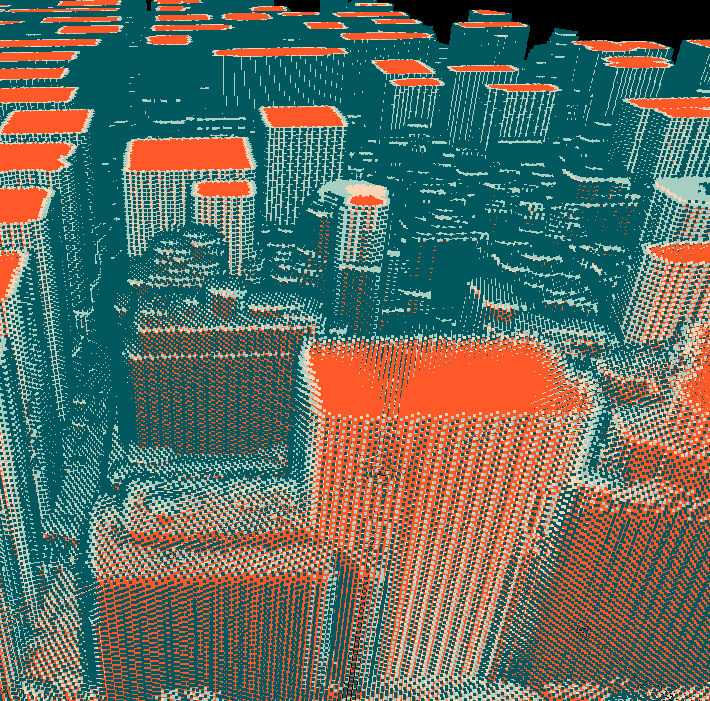
\includegraphics[width=0.5\linewidth]{chapter_5_mapping/imgs/voxel_map_ny_2.png}
  \caption[Example occupancy and risk map of New York City]{Example occupancy and risk map of New York City. Obstacles are colored orange with a surrounding potential field denoted by pink, light blue, and dark blue colors. Buildings which do not fit in the map (higher then 400 feet AGL), are shown with orange roofs.}
  \label{fig:ch5_ny_voxel_map}
\end{figure}

An A* path planner is used to generate optimal collision free trajectories inside $R_{map}$. Obstacle nodes, cells with a value of 255, are ignored for state transitions. The risk function described in Eq. \ref{eq:ch5_risk_function_planner} is defined as
\begin{equation}
\text{risk}(i,j,k) = \frac{R_{map}(i,j,k )}{255} 
\end{equation}
The path risk to a goal cell, $n_g$, is the path cost to the goal node normalized by $R$
\begin{equation}
r_p = \frac{g(n_g)}{R} 
\end{equation}


% \subsection{Path Planning Algorithm}\label{sec:ch5_path_planner}

% Optimal planning algorithms require a cost function to explore the search space in pursuit of a feasible and optimal solution. For discrete search planners, the space must first be discretized into a graph ${G}({V},{E})$, where ${V}$ denotes the vertices with corresponding edge set ${E}$ expressing vertex transitions and their path cost. This graph is defined implicitly for the 3D occupancy and risk map $R_{map}$. The vertices are the cells/voxels in $R_{map}$ accessed with 3 tuple indices $(i,j,k)$. The edge set (including path cost) of each cell is dynamically computed from the 26 neighbors which surround it. Obstacle nodes, cells with a value of 255, are ignored for state transitions.

% An A* path planner was used to validate the proposed emergency landing planning framework. The implemented planning scheme traded off between paths resulting in high risk to the aircraft (i.e., flying to close to nearby buildings) and the distance of travel required.  The multidimensional risk map defined above, $R_{map}$, is used by our A* path planner to generate optimal collision free paths from the current \ac{UAS} position to a landing site. A* is used with cost $g(n)$ and heuristic  $h(n)$ functions calculated as
% \begin{align}
%     c(n', n) &= \text{dist}(n', n) 
%     \cdot (1 + \text{risk}(n)) \\
%     g(n) &= g(n') + c(n, n')\\
%     h(n) &= \text{dist}(n, goal)\\
%     f(n) &= g(n) + h(n)
% \end{align}
% where $c$ is the transition cost between the current node $n$ and the previous node $n'$, $g$ is the cumulative cost, $h$ is the heuristic cost, $f$ is the estimated total cost, $\mathbf{dist}(\cdot)$ calculates the distance between nodes, and $\mathbf{risk}(\cdot)$ returns the normalized risk encoded in $R_{map}$. Once a path is found to the goal, the path risk, $r_p$, is the total accrued cost of the path to reach the goal node normalized by $R$.


\begin{figure}[!t]
  \centering
  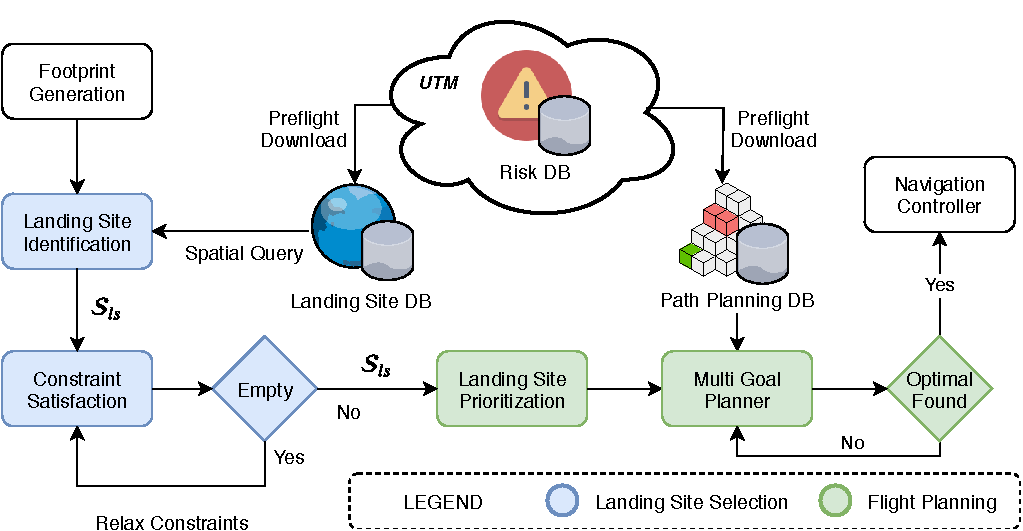
\includegraphics[width=0.75\linewidth]{chapter_5_mapping/imgs/architecture_planning.pdf}
  \caption{Flow chart of proposed map-based planner.}
  \label{fig:ch5_architecture_overview}
\end{figure}


\section{Planning Risk Metric Analysis and Integration}\label{sec:ch5_mapbased_planner}
Section \ref{sec:ch5_architecture_planner} describes the architecture of our proposed map-based planner. Section \ref{sec:ch5_trade-off} outlines the inherent trade-off between landing site and path risk and our planning method. Section \ref{sec:ch5_multi_goal_search_all} provides underlying theoretical and algorithmic formulations of our multi-goal planner.

\subsection{Real-time Map-Based Planner Architecture}\label{sec:ch5_architecture_planner}

The proposed architecture for our map-based planner is shown in Figure \ref{fig:ch5_architecture_overview} which is modified from our previous work \cite{atkins_emergency_2006, castagno_comprehensive_2018}. The landing site and path planning database might be provided as part of NASA's \ac{UAS} Traffic Management (UTM) service \cite{prevot_uas_2016}. Before mission operations begin, a preflight download commences from UTM servers to retrieve relevant data for the flight operational area.  These data are lightweight thus can be stored onboard the UAS. 
In the event an urgent landing situation arises our map-based planner logic will be executed. First a footprint specifying the bounds of the reachable landing area is generated. Construction of such a footprint is not the focus of this chapter, however work by \cite{paul_flight_2017, atkins_emergency_2006} and \cite{ten_harmsel_emergency_2017} have investigated its generation for fixed-wing and multicopter aircraft, respectively. For simplification our footprint is a circle of radius $R$ whose center is the \ac{UAS} position. Next we efficiently query the spatially indexed landing site database to provide the set of risk-evaluated landing sites $\mathcal{S}_{ls}$. Landing sites are filtered by user defined constraints such as landing site height or area. If no valid landing sites are found constraints are relaxed as needed.

The planner must identify a low risk landing site and flight plan  from the set of candidate landing sites $\mathcal{S}_{ls}$.  In order to assess each landing site's path risk the physical path to each landing site is needed. Optimal collision-free path planning in three dimensional space can take a significant amount of time thus is impractical to perform in real-time for the numerous potential landing sites that may be available for a small \ac{UAS} in a city environment. Therefore we use a heuristic to prioritize landing sites in $\mathcal{S}_{ls}$ by minimum total risk. This sorted list is then sent to our multi-goal planner which efficiently searches over landing sites until the risk-optimal landing site/path pair is found. Finally the landing site and path is sent to a navigation controller. 
% Section \ref{sec:ch5_multi_goal_search_all} details our multi-goal planner.

\subsection{Trade-off Between Landing Site and Path Risk}\label{sec:ch5_trade-off}
% The map-based planner must identify the optimal landing site and flight plan pair from the set of candidate landing sites $\mathcal{S}_{ls}$.
Minimizing the landing site risk and path risk to a site requires solving a multi-objective (MO) optimization problem from which there may not be a single solution simultaneously optimal over both objectives. An analysis of trade-offs is required for MO problems by computing and analyzing a Pareto frontier. Frontier visualization aids system designers in choosing the relative weighting of objective trade-offs to select a single ``best'' solution \cite{ngatchou_pareto_2005}. 

\begin{figure}[h!]
\centering
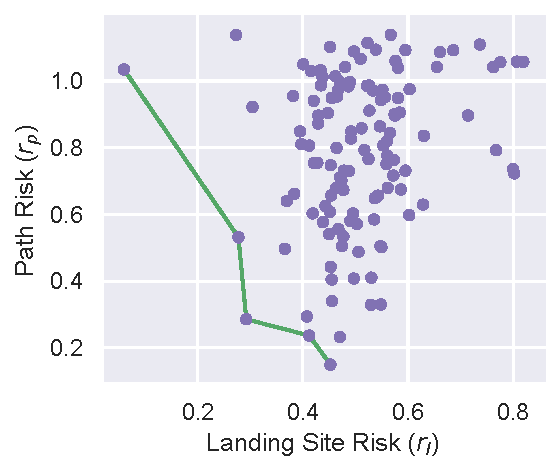
\includegraphics[width=.5\linewidth]{chapter_5_mapping/imgs/witten_Scenario1_pareto.pdf}
\caption[Example Pareto frontier for landing site and path risk]{Example Pareto frontier for landing site and path risk. Demonstrates trade-off between to minimize both objectives. Points in the Pareto frontier are connected by a green line.}
\label{fig:ch5_pareto_example}
\end{figure}

Fig. \ref{fig:ch5_pareto_example} shows an example Pareto frontier that minimizes two objectives: landing site risk and path risk.  Each purple dot represents a landing site. The $x$-axis represents landing site risk and the $y$-axis represents path risk to that site. 
% The path risk is it's path cost (length and potential field penalties) normalized by $R$. 
% The graph by itself makes no determination of the weighting or ``worth'' between the two objectives.  
The green line connects three points on the Pareto frontier, the set of non-dominated landing sites for which any improvement in one objective results in a negative trade-off in the other. Each of these three landing sites is ``optimal'', and a quantifiable relationship between each objective must be constructed to select a final choice. A linear weighting scheme between the objectives is proposed below for each landing site $l_i \in \mathcal{S}_{ls} $:
\begin{equation}\label{eq:ch5_total_risk}
    r_{t} = w_l \cdot r_{l} + w_p \cdot r_{p}
\end{equation}
where $r_{t}$ refers to the total risk and $w_l$ and $w_p$ are weights for landing site risk and path risk, respectively. The optimal landing site can then be found by solving the optimization problem shown in Eq. \ref{eq:ch5_optimization}.
\begin{equation}
    l_{i^*} = \argminA_{l_i \; \in \; \mathcal{S}_{ls}} \; r_{t}\label{eq:ch5_optimization}
\end{equation}

\subsection{Multi-Goal Planner}\label{sec:ch5_multi_goal_search_all}

Our multi-goal planner selects a landing site that minimizes total risk given a user-defined weighted trade-off between landing site risk and path risk. Each landing site's position and risk is assumed known \emph{a priori}. Path risk cannot be known until the physical path is computed. Because this work relies on preprocessed map data rather than real-time perception, path planning has the highest real-time computational overhead.
Multi-goal search allows exploration of many low-risk landing sites but will be computationally expensive. Our planner efficiently prunes high risk goals/paths from the search space to reduce computational overhead.  Ultimately the planner returns one goal/path pair minimizing combined total risk.
The algorithm begins by creating an array of landing site data structures with the following form:
\begin{align}
    l_i = \{ \mathbf{c},\; r_{l}, \;r_{p}, \; r_{t,min}, \; found \} \\
    \mathbf{c} \in \mathbb{R}^3 \\
    r_{l}, r_{p}, r_{t,min} \in \mathbb{R} \\
    found \in \{\; 0, 1 \; \} 
\end{align}
where $\mathbf{c}$ is landing site position, $r_{l}$ is landing site risk, $r_{p}$ is path risk, $r_{t,min}$ is minimum total risk, and $found$ is a Boolean indicating whether a path has been found to landing site $i$. The minimum
total risk is computed from

\begin{equation}
    r_{t,min} = w_{l} \cdot r_{l} + w_p \cdot  h(\mathbf{O}_{UAS}, \mathbf{c}) / R
\end{equation}
where $h()$ is an admissible heuristic, 3D octile distance in this work. We access elements in $l_i$ through dot (\textbf{.}) notation, e.g. $l_i.r_{t,min}$ refers to the minimum total risk of the $i^{th}$ landing site in $\mathcal{S}_{ls}$. Section \ref{sec:ch5_theorom} provides definitions and a theorem for our multi-goal planner. Section \ref{sec:ch5_alg_impl} describes the planning algorithm and its implementation.

\subsubsection{Theory}\label{sec:ch5_theorom}


\begin{definition}{Total Ordered Set}\label{def:total_order}
Binary relation, $\le$, is a total order on set $\mathcal{X}$ if $\forall a,b \; \in \mathcal{X}$
\begin{enumerate}
    \item $a \le b$ and $b \le a \implies a = b$ \quad Anti-symmetry
    \item $a \le b$ and $b \le c \implies a \le c$ \quad Transitivity
    \item $a \le b$ or $b \le a$  \quad Connexity
\end{enumerate}
\end{definition}
We define binary operator $\le$ on the set $\mathcal{S}_{ls}$  $\forall l_i,l_j \in \mathcal{S}_{ls}$:
\begin{equation}
    l_{i} \le l_{j} : l_{i}.r_{t,min} \le l_{j}.r_{t,min}
\end{equation}
This operator is used to sort $\mathcal{S}_{ls}$ such that the natural numbers $i,j \in [1, N]$ index with the following property:
\begin{align}
   \forall l_i, l_j \in \mathcal{S}_{ls} \; l_i \le l_j \iff i \le j
\end{align}
where $N = |\mathcal{S}_{ls}|$. We use bracket operator \textbf{[$\cdot$]} to index $\mathcal{S}_{ls}$, e.g., $l_i = {S}_{ls}[i]$.

\begin{theorem}\label{thm:ch5_thm1}
Let $i^{*} \in [1, N]$ and $k \in [1, N]$ be natural numbers where $i^* \le k$.  If $\forall j \in [1, k],\; l_{i^{*}}.r_{t} \le l_j.r_{t}$ and  $l_{i^{*}}.r_{t} \le l_{k+1}.r_{t,min}$  then $l_{i^{*}}$ has the minimum total risk: 
\begin{equation}
    l_{i^{*}} = \argminA_{l_i \; \in \; \mathcal{S}_{ls}} \; l_i.r_{t}
\end{equation}

\end{theorem}

\begin{proof}

% Theorem \ref{thm:ch5_thm1} logical implication rests upon two clauses in the antecedent:
% \begin{enumerate}
%     \item $\forall j \in [1, k] \; l_{i^{*}}.r_{t} \le l_j.r_{t}$.
%     \item $l_{i^{*}}.r_{t} \le l_k.r_{t,min}$.
% \end{enumerate}
The stated inequalities partition $\mathcal{S}_{ls}$ into two ordered sets for some index $k \in [1, N]$. We denote $\mathcal{S}_{ls}^{low} = \{l_1, \dots, l_k \}$ where $l_{i^{*}} \in \mathcal{S}_{ls}^{low}$ and $\mathcal{S}_{ls}^{hi} = \{l_{k+1}, \dots , l_N\} \cup \{l_{i^{*}}\}$. We must show that $l_{i^{*}}$ represents the minimum total risk in both sets. When $\forall j \in [1, k] \; l_{i^{*}}.r_{t} \le l_{j}.r_{t}$ holds true, by the definition of argmin we know that:
\begin{flalign*}
    (1) && l_{i^*} = \argminA_{l_i \; \in \; \mathcal{S}_{ls}^{low}} l_i.r_{t}
\end{flalign*}
To show $l_{i^*}$ has the minimum actual total risk of $\mathcal{S}_{ls}^{hi}$ we begin by noting that for each landing site $l_j$ 
\begin{flalign*}
    (2) \hfill && \forall j \in [1, N], \; l_{j}.r_{t,min} \le l_{j}.r_{t} 
\end{flalign*}
If a landing site $l_i$ has total risk $l_i.r_t$ which is less than the minimum total risk of landing site $l_j$ denoted $l_j.r_{t,min}$ then
\begin{flalign*}
    (3) && \forall\; i,j \in [1, N] \; l_{i}.r_{t} \le l_{j}.r_{t,min} \implies  l_{i}.r_{t} \le l_{j}.r_{t} 
\end{flalign*}
From the transitivity property of $\mathcal{S}_{ls}$ we obtain
\begin{flalign*}
(4) && \exists \;i^{*}, k \in [1, N] \; s.t. \; l_{i^{*}}.r_{t} \le l_{k+1}.r_{t,min} \implies \forall j \in [k+1, N] \; l_{i^{*}}.r_{t} \le l_j.r_{t,min} 
\end{flalign*}
Finally by combining (3) and (4) we obtain
\begin{flalign*}
(5) && \exists \;i^{*}, k \in [1, N] \; s.t. \; l_{i^{*}}.r_{t} \le l_{k+1}.r_{t,min} \implies \forall j \in [k+1, N] \; l_{i^{*}}.r_{t} \le l_j.r_{t} % Syllogism
\end{flalign*}
Using the definition of argmin we restate (5) as
\begin{flalign*}
(6) && \exists \;i^{*}, k \in [1, N] \; s.t. \; l_{i^{*}}.r_{t} \le l_{k+1}.r_{t,min} \implies l_{i^*} = \argminA_{l_i \; \in \; \mathcal{S}_{ls}^{hi}} l_i.r_{t}
\end{flalign*}

% \begin{align*}
%     (2) && \forall j \in [1, N] \; l_{j}.r_{t,min} \le l_{j}.r_{t} \\
%     (3) && \forall\; i,j \in [1, N] \; l_{i}.r_{t} \le l_{j}.r_{t,min} \implies  l_{i}.r_{t} \le l_{j}.r_{t} \\
%     (4) && \exists \;i^{*}, k \in [1, N] \; s.t. \; l_{i^{*}}.r_{t} \le l_{k+1}.r_{t,min} \implies \forall j \in [k+1, N] \; l_{i^{*}}.r_{t} \le l_j.r_{t,min} \\
%     (5) && \exists \;i^{*}, k \in [1, N] \; s.t. \; l_{i^{*}}.r_{t} \le l_{k}.r_{t,min} \implies \forall j \in [k, N] \; l_{i^{*}}.r_{t} \le l_j.r_{t} \\ % Syllogism
%     (6) && \exists \;i^{*}, k \in [1, N] \; s.t. \; l_{i^{*}}.r_{t} \le l_{k}.r_{t,min} \implies l_i^{*} = \argminA_{l \; \in \; \mathcal{S}_{ls}^{hi}} l.r_{t}
% \end{align*}
Statements (1) and (6) show that $l_{i^{*}}$ has the minimum total risk in $\mathcal{S}_{ls}^{low}$ and $\mathcal{S}_{ls}^{hi}$ if both qualifying predicates hold true. Therefore the union of these sets, $\mathcal{S}_{ls}$, has the same minimum $l_{i^{*}}.r_t$. 

% Equation \ref{eq:ch5_array_end} states that \emph{if} a landing site at index $i$ in $\mathcal{S}_{ls}$ has a lower total risk than the \emph{minimum} total risk of landing site $k$ then $i$ will have lower risk than all elements downstream of $k$ in the array. To show that $i$ index
\end{proof}

\begin{remark}
There may \emph{not} exist a $k$ for which the second clause $l_{i^{*}}.r_{t} \le l_{k+1}.r_{t,min}$ in Theorem \ref{thm:ch5_thm1} holds true. In this case $\mathcal{S}_{ls}^{low} = \mathcal{S}_{ls}$ and path planning must be performed for every landing site to guarantee risk-optimality.
\end{remark}


\subsubsection{Multi-goal Path Planning Algorithm}\label{sec:ch5_alg_impl}

Our multi-goal path planner is shown in Algorithm \ref{alg:ch5_multi_goal}.  First, $\mathcal{S}_{ls}$ is sorted by minimum total risk as described in Definition \ref{def:total_order}.  The algorithm next initializes variables $\hat{l}_{min}, \hat{p}_{min},$ and $\hat{r}_{t}$ to track the minimum risk landing site, associated path, and total risk, respectively. These variables represent the current best landing site/path pair and are updated each time a lower risk landing site is found. 

Our algorithm repeatedly investigates the next most promising landing site $l_i$ from $\mathcal{S}_{ls}$. Line 11 starts a path planning sequence with 3D octile distance heuristic guiding the planner to $l_i$. The planner is opportunistic so that other landing sites (goals) may be found during the search.  For this reason the identified landing site is returned from function \texttt{PathPlanning}, $l_j$, and will not always be equal to $l_i$. The true total risk of $l_j$ is then calculated for the full flight plan and its \emph{found} flag set. This landing site's total risk is then compared to the current best and updated if appropriate, ensuring the first clause of Theorem \ref{thm:ch5_thm1} is satisfied.

The first element in $\mathcal{S}_{ls}$ which has not been found is returned in Line 18 as the next unplanned landing site that has minimum total risk. The tracked total risk is compared with this element's minimum total risk, and if less or equal will satisfy the second clause in Theorem \ref{thm:ch5_thm1}. Once both predicates are satisfied iteration terminates and $\hat{l}_{min}$, $\hat{p}_{min}$ are returned as the risk-optimal landing site and plan, respectively. 
% This is the confusing part (below here)
If the optimal site is not found then the procedure continues. Line 21 ensures that if $l_i$ was not found ($l_j$ is \emph{not} $l_i$) then the planner will retry $l_i$ in the next iteration. This is accomplished by decrementing the loop variable $i$. The total number of iterations is equal to $k$ in Theorem \ref{thm:ch5_thm1} which represents the number of landing sites searched.

Note that the algorithm can return the best found landing site and path at any iteration step if computational time becomes a concern. In addition a worst case bound of unnecessary risk can be computed from the difference between the returned landing site's total risk and the minimum total risk of the next landing site to be searched.

\SetKwRepeat{Struct}{struct \{}{\}}%
\newcommand{\Float}{\KwSty{float}}
\newcommand{\Vecthree}{\KwSty{vec3f}}
\newcommand{\Boolean}{\KwSty{bool}}
\newcommand{\forcond}{$i=0$ \KwTo $n$}


\begin{algorithm}[!t]
    \SetKwInOut{Input}{Input\hspace{0.3cm}}
    \SetKwInOut{Output}{Output}

    \Input{\hspace{0.0cm}Landing Site Set ($\mathcal{S}_{ls}$), \\ Map ($M$), \\ UAS Location ($\mathbf{O}_{UAS}$) \\ Footprint Radius ($R$), \\  Weighting Trade-off ($ w_{l}, w_p $), \\  Heuristic ($h(c_i, c_j)$)}
    
    \Output{\hspace{0.0cm}Best landing site and path, $\hat{l}_{min}$ and $\hat{p}_{min} $}
    
    $\mathcal{S}_{ls}$ = $\operatorname{LandingSitePrioritization}(\mathcal{S}_{ls}, \mathbf{O}_{UAS}, R, w_{l}, w_p, h)$ \\
    $N$ = $\vert\;\mathcal{S}_{ls}\;\vert$ \\
    $\hat{l}_{min} = None$\\
    $\hat{p}_{min} = None$\\
    $\hat{r}_{t} = \infty$\\
    \For{$i=0$ \KwTo $N$}{
        $l_i = \mathcal{S}_{ls}[i]$ \\
        \uIf{$l_i$.found}{
            continue
        }
        $goals = \{\forall \; l_i \in \ \mathcal{S}_{ls}\; | \; not \; l_i.found \}$  \\
        $l_j, p_j$ = PathPlanning($M, \mathbf{O}_{UAS}, R, h, l_i, goals$)\\
        $l_j$.found = true \\
        $l_j$.$r_{t}$ = $w_{l} \cdot l_j$.$r_{l} + w_p \cdot \frac{\operatorname{Cost}(p_j)}{R}$ \\
        \uIf{$l_j.r_{t} < \hat{r}_{t}$}{
            $\hat{r}_{t} = l_j.r_{t}$ \\
            $\hat{l}_{min} = l_j$ \\
            $\hat{p}_{min} = p_j$ 
        }
        $l_{n} = \operatorname{FirstElement}(\{\forall \; l_i \in  \mathcal{S}_{ls}\; | \; not \; l_i.found  \}$)  \\
        \uIf{$\hat{r}_{t} <= l_n.{r}_{t,min}$}{
            break
        }
        \uIf{not $l_i$.found}{
            i = i - 1
        }
    }
    return $\hat{l}_{min}, \hat{p}_{min}$
    \caption{Multi-Goal Search}
    \label{alg:ch5_multi_goal}
\end{algorithm}


\section{Maps and Simulation Results}\label{sec:ch5_experiments}

Landing site databases and path planning obstacle maps were generated for the cities of Ann Arbor, Michigan; Witten, Germany; and mid-town Manhattan, New York City, New York using the methods outlined in Sections \ref{sec:ch5_landing_site_database} and \ref{sec:ch5_occupancy_map}. Public data sources used for all three cities are shown in Table \ref{table:ch5_data_sources}. Visualization and analysis of each city's databases and maps are found in Section \ref{sec:ch5_generated_maps}. Section \ref{sec:ch5_case_studies} presents two urgent landing scenarios for each city with results from our proposed framework. Section \ref{sec:ch5_meta_analysis} provides statistical analysis of our planners speed and efficacy in all three cities. Table \ref{table:ch5_weights} displays parameters used throughout all case studies and simulations. The average touchdown site areas $A_{avg}$ in each city were set to 150, 100, and 100 square meters for Ann Arbor, Witten, and New York respectively. The minimum touchdown radius and corresponding area were set to 2 meters and 12.5 square meters, respectively, for all cases.

\begin{table}[ht]
\centering
\caption{Satellite, LiDAR, and Building Data Sources}\label{table:ch5_data_sources}
\begin{tabular}{c@{\qquad}cc@{\qquad}cc@{\qquad}c}
  \hline\noalign{\smallskip}
  City & Satellite & LiDAR & Buildings \\
  \hline\noalign{\smallskip}
  Ann Arbor & Bing \cite{satellite_annarbor}            & USGS \cite{usgs_lidar_2018-annarbor}       & \ac{OSM}\cite{openstreetmap_contributors_planet_2017}  \\
  Witten    & Land NRW \cite{satellite_germany}         & Open NRW \cite{lidar_germany}    & \ac{OSM}\cite{openstreetmap_contributors_planet_2017}  \\
  New York  & New York State \cite{satellite_newyork}   & USGS \cite{usgs_lidar_2018_ny}        & \ac{OSM}\cite{openstreetmap_contributors_planet_2017}  \\
\noalign{\smallskip}\hline\noalign{\smallskip}
\end{tabular}
\end{table}


\begin{table}[ht]
\centering
\caption[Emergency Landing Case Study Parameters]{All Case Study Parameters}
\label{table:ch5_weights}
\begin{tabular}{@{}llll@{}}
\hline\noalign{\smallskip}
Group                                           & Parameter    & Value                     & Description                \\ 
\noalign{\smallskip}\hline\noalign{\smallskip}
\multirow{3}{*}[10pt]{Landing Site Risk}        & $w_v$         & 0.8                       & Weight for vehicle cost    \\
                                                & $w_s$        & 0.2                       & Weight for property cost \\
                                                & $w_o$        & 0.0                       & Weight for human occupancy cost   \\
\multirow{3}{*}[10pt]{Vehicle Cost}        & $w_t$         & 0.4                       & Weight for terrain type cost    \\
                                                & $w_a$        & 0.4                       & Weight for area cost \\
                                                & $w_{ca}$        & 0.2                       & Weight for cumulative area cost   \\
\multirow{3}{*}[10pt]{Multi-Goal Planner}       & $w_l$        & 0.6                       & Weight for landing site risk    \\
                                                & $w_p$        & 0.4                       & Weight for path risk   \\
                                                & $R$        & 250m                       & Search radius footprint   \\
\noalign{\smallskip}\hline\noalign{\smallskip}
\end{tabular}
\end{table}

\subsection{Landing Sites and Risk Maps}\label{sec:ch5_generated_maps}

Figure \ref{fig:ch5_all_ls_risk} shows extracted landings sites and their associated risks for the cities of Ann Arbor (a), Witten (b), and New York (c). Landing site risk is color-coded from low (light yellow) to high (dark orange). Touchdown sites are displayed as blue circles.
% Most landing sites in these cities are flat rooftops that are marked appropriate for landing given our proposed methods. 
The operating regions are approximately $1500\times1500$, $1500\times1300$, and $1500\times3000$ meters for Ann Arbor (AA), Witten (WT), and New York (NY), respectively. Three-dimensional risk grids as described in Section \ref{sec:ch5_occupancy_map} were generated for all three cities. Each voxel in $R_{map}$ is a cube with two meter edge length. This resolution provides a balance between file size and providing sufficient resolution for use in path planning. The resulting file sizes are approximately 37, 26, and 67 MB for AA, WT, and NY respectively.

\begin{figure}[!t]
 \centering
 \begin{minipage}[b]{0.50\textwidth}
   \begin{subfigure}[b]{\linewidth}
    \centering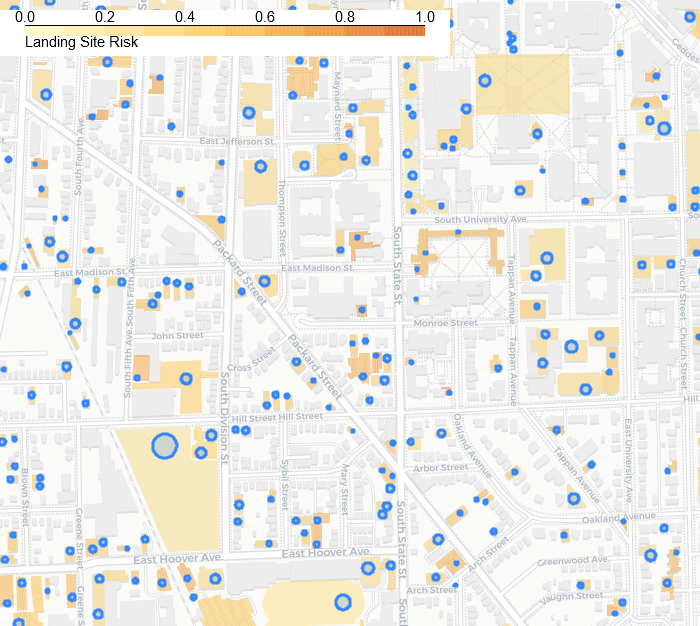
\includegraphics[clip, trim=0.0cm 0.0cm 0.0cm 0.0cm, width=\linewidth]{chapter_5_mapping/imgs/annarbor_all_ls_risk.png}
     \caption{Ann Arbor}\label{fig:ch5_aa_all_risk}
   \end{subfigure}\\[\baselineskip]
   \begin{subfigure}[b]{\linewidth}
    \centering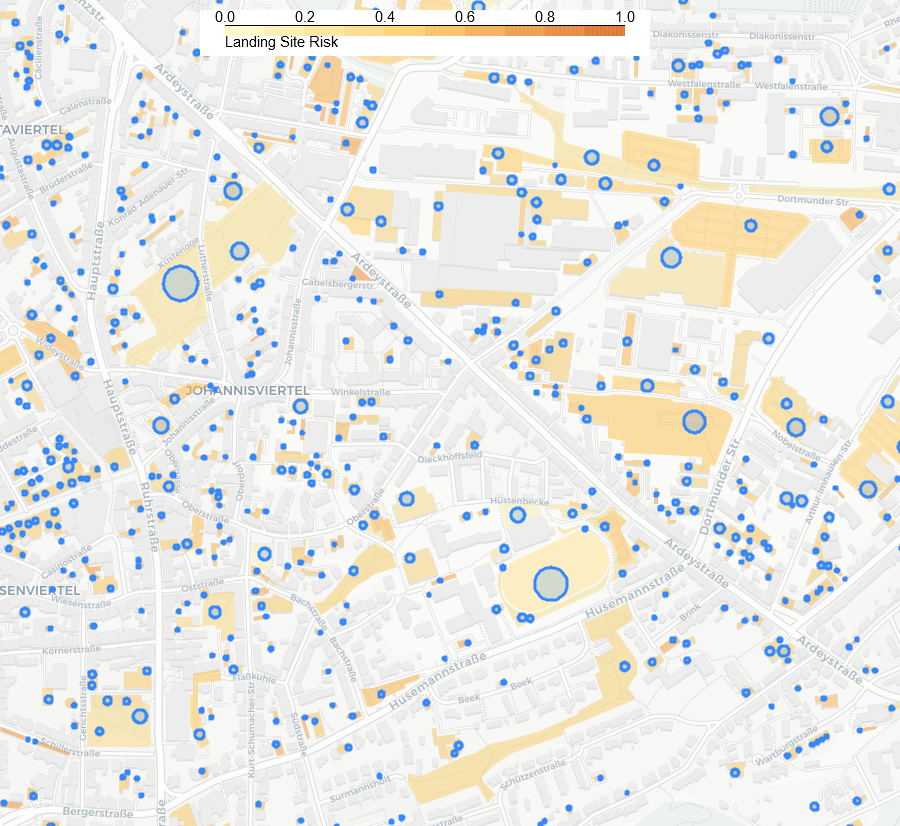
\includegraphics[clip, trim=0.0cm 0.0cm 0.0cm 0.0cm, width=\linewidth]{chapter_5_mapping/imgs/witten_all_ls_risk.png}
     \caption{Witten}\label{fig:ch5_wt_all_risk}
   \end{subfigure}
 \end{minipage}
 \hfill
 \begin{subfigure}[b]{0.44\textwidth}
 \centering
 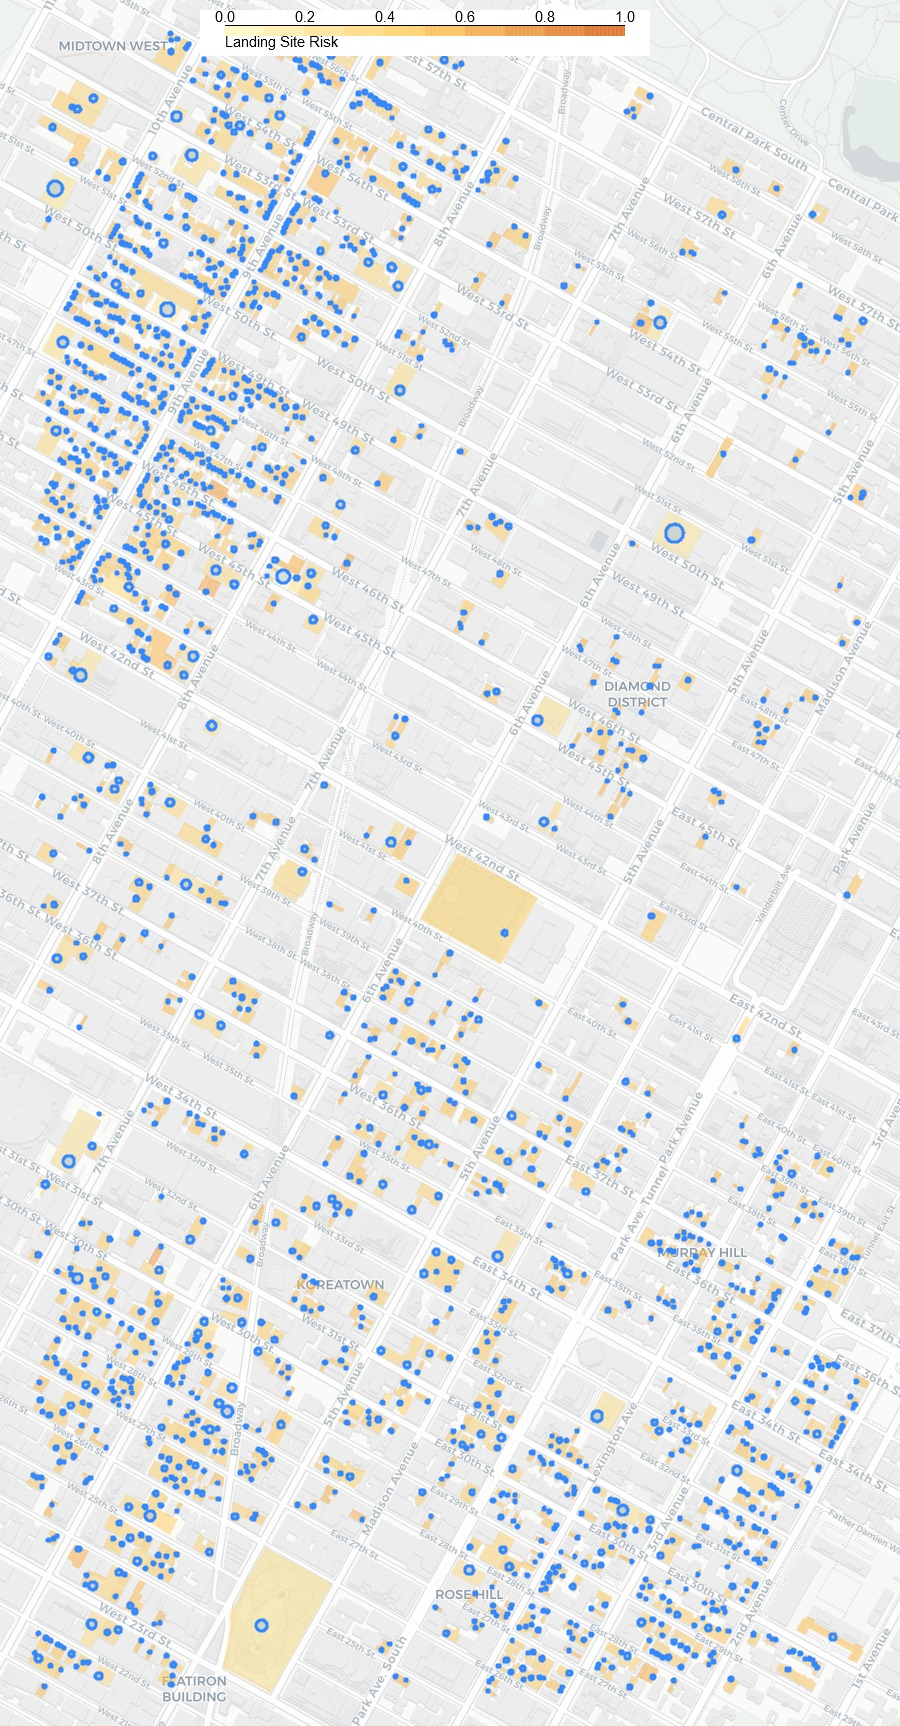
\includegraphics[clip, trim=0.0cm 0.0cm 0.0cm 0.0cm, width=\linewidth]{chapter_5_mapping/imgs/newyork_all_ls_risk.jpg}
%   \rule{\linewidth}{\dimexpr 2\linewidth+2\baselineskip+6pt}
   \caption{New York}\label{fig:ch5_ny_all_risk}
 \end{subfigure}
 \caption[Maps of landing sites and associated risk.]{Maps of landing sites and associated risk. Landings site risk for the cities of Ann Arbor (a), Witten (b), and New York (c). Landing sites are color-coded from low risk (light yellow) to high risk (dark orange). Touchdown sites are denoted by blue circles. Maps from \copyright OpenStreetMap contributors and \copyright CARTO. License: Open Database License: https://www.openstreetmap.org/copyright}\label{fig:ch5_all_ls_risk}
\end{figure}


\subsection{Case Studies}\label{sec:ch5_case_studies}

We present two case studies for each city where an urgent landing is required for a small UAS.  Figure \ref{fig:ch5_all_scenarios_map} presents a map of each case study with locations shown in Table \ref{sec:ch5_case_studies}. The first row (a,b) is for Ann Arbor, the second row (c,d) is for Witten, and the final row (e,f) is for Manhattan. Position of the \ac{UAS} during the urgent landing event is indicated by the green marker. Landing site risk is colorized from low (yellow) to high (dark orange) risk with associated touchdown sites marked as blue circles. The lowest risk landing sites, not considering path risk, are ranked and marked with blue numbered icons. Our planner's chosen landing site is marked in red which trades off landing site and path risk. 
Pareto plots are also provided for each of these case studies in Fig. \ref{fig:ch5_all_pareto_plots}. To generate these plots, collision-free paths to \textit{all} landing sites for each scenario were generated, providing their actual path risk. The first, second, and third row correspond to Ann Arbor, Witten, and New York, respectively.  Each scenario graph has the same axis limits, allowing the reader to compare each scenario visually. Each purple dot represents a landing site, while the red dot represents the landing site chosen by the map-based planner. The Pareto set for each scenario is depicted by the green line. 


\begin{figure}[!ht]
    \centering
      \begin{subfigure}[b]{0.47\linewidth}
        \centering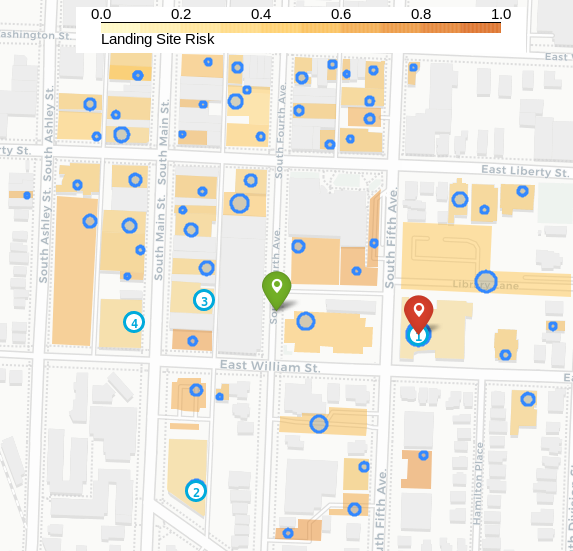
\includegraphics[clip, width=155pt, height=130pt]{chapter_5_mapping/imgs/annarbor_scenario_2.png}
        \caption{\label{fig:ch5_aa_map1}}
      \end{subfigure}
      \begin{subfigure}[b]{0.47\linewidth}
        \centering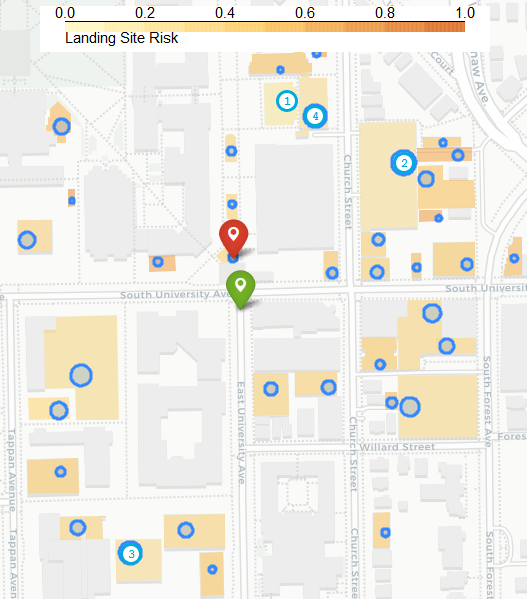
\includegraphics[width=155pt, height=130pt]{chapter_5_mapping/imgs/annarbor_scenario_4.png}
        \caption{\label{fig:ch5_aa_map2}}
      \end{subfigure}
      \begin{subfigure}[b]{0.47\linewidth}
        \centering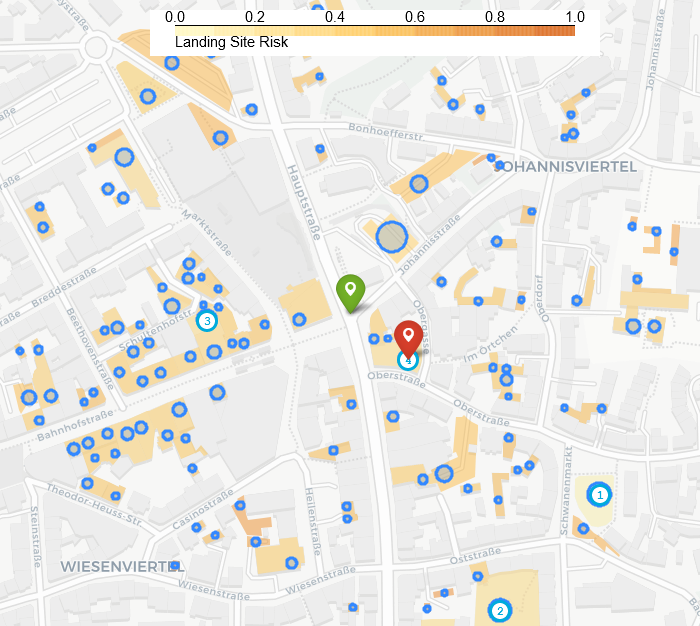
\includegraphics[clip, width=155pt, height=130pt]{chapter_5_mapping/imgs/witten_scenario_1.png}
        \caption{\label{fig:ch5_wt_map1}}
      \end{subfigure}
      \begin{subfigure}[b]{0.47\linewidth}
        \centering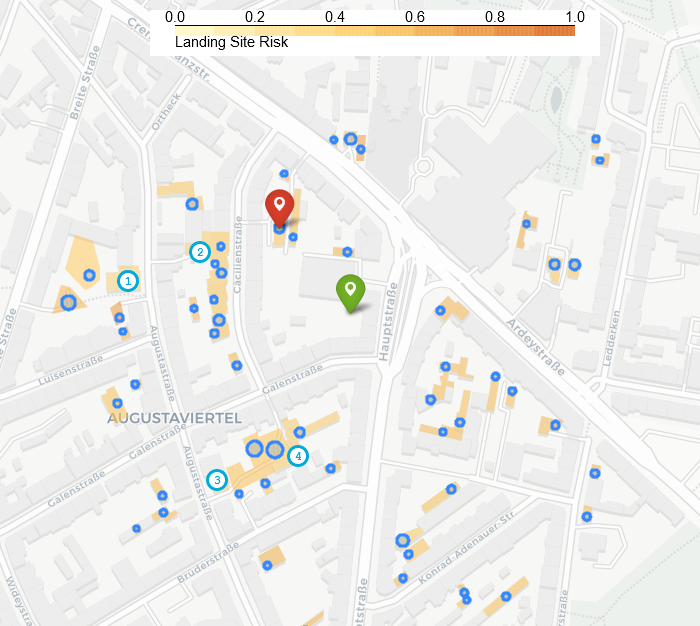
\includegraphics[width=155pt, height=130pt]{chapter_5_mapping/imgs/witten_scenario_2.png}
        \caption{\label{fig:ch5_wt_map2}}
      \end{subfigure}
      \begin{subfigure}[b]{0.47\linewidth}
        \centering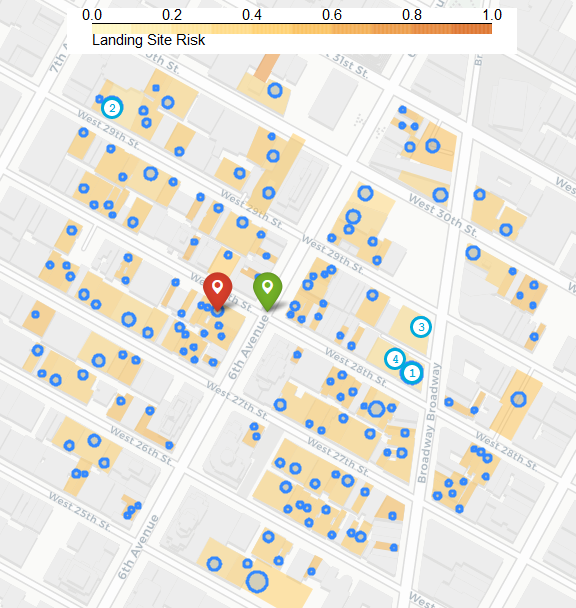
\includegraphics[clip, width=155pt, height=130pt]{chapter_5_mapping/imgs/newyork_scenario_1.png}
        \caption{\label{fig:ch5_ny_map1}}
      \end{subfigure}
      \begin{subfigure}[b]{0.47\linewidth}
        \centering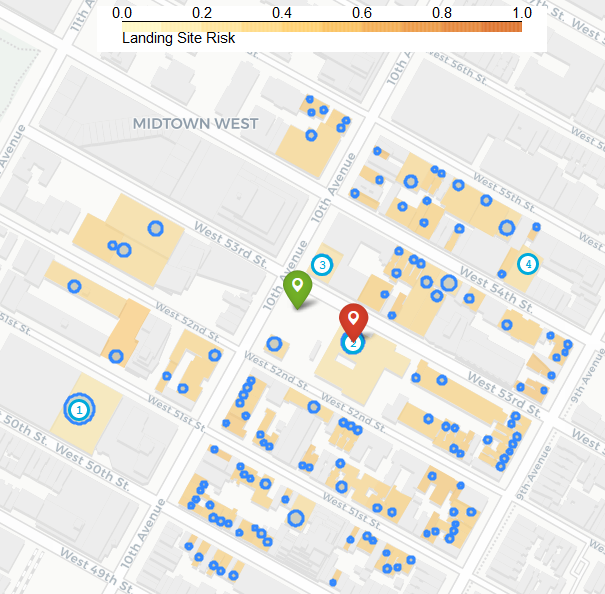
\includegraphics[width=155pt, height=130pt]{chapter_5_mapping/imgs/newyork_scenario_4.png}
        \caption{\label{fig:ch5_ny_map2}}
      \end{subfigure}
         \caption[Maps of case studies for emergency landing]{Maps of case studies for emergency landing. Maps of Ann Arbor (a,b), Witten (c,d), and New York (e, f).  Failure position of the \ac{UAS} is indicated by the green marker. Landing site risk is colorized from low (yellow) to high (dark orange) risk, with associated touchdown sites marked as blue circles. The lowest risk landing sites are ranked and marked with blue numbered icons. Our planner's chosen landing site is marked in red which trades off landing site and path risk. Maps from \copyright OpenStreetMap contributors and \copyright CARTO. License: Open Database License: https://www.openstreetmap.org/copyright}
     \label{fig:ch5_all_scenarios_map}
\end{figure}

\begin{table}[ht]
\centering
\caption[Emergency Landing Case Study Locations]{Case Study Locations}
\label{table:ch5_case_studies}
\begin{tabular}{c@{\qquad}c@{\qquad}c}
\hline\noalign{\smallskip}
Scenario   & Lng/Lat (degrees)        & Height, MSL (m)  \\
\noalign{\smallskip}\hline\noalign{\smallskip}
AA CS\#1    & 42.2783, -83.7473  & 260          \\
AA CS\#2    & 42.2748, -83.7357   & 270          \\
WT CS\#1    & 51.4391, 7.3369   & 109          \\
WT CS\#2    & 51.4443, 7.3359   & 130          \\
NY CS\#1    & 40.7460, -73.9905   & 19         \\
NY CS\#2    & 40.7662, -73.9903   & 17         \\
\noalign{\smallskip}\hline\noalign{\smallskip}
\end{tabular}
\end{table}

\begin{figure}[t]
    \centering
    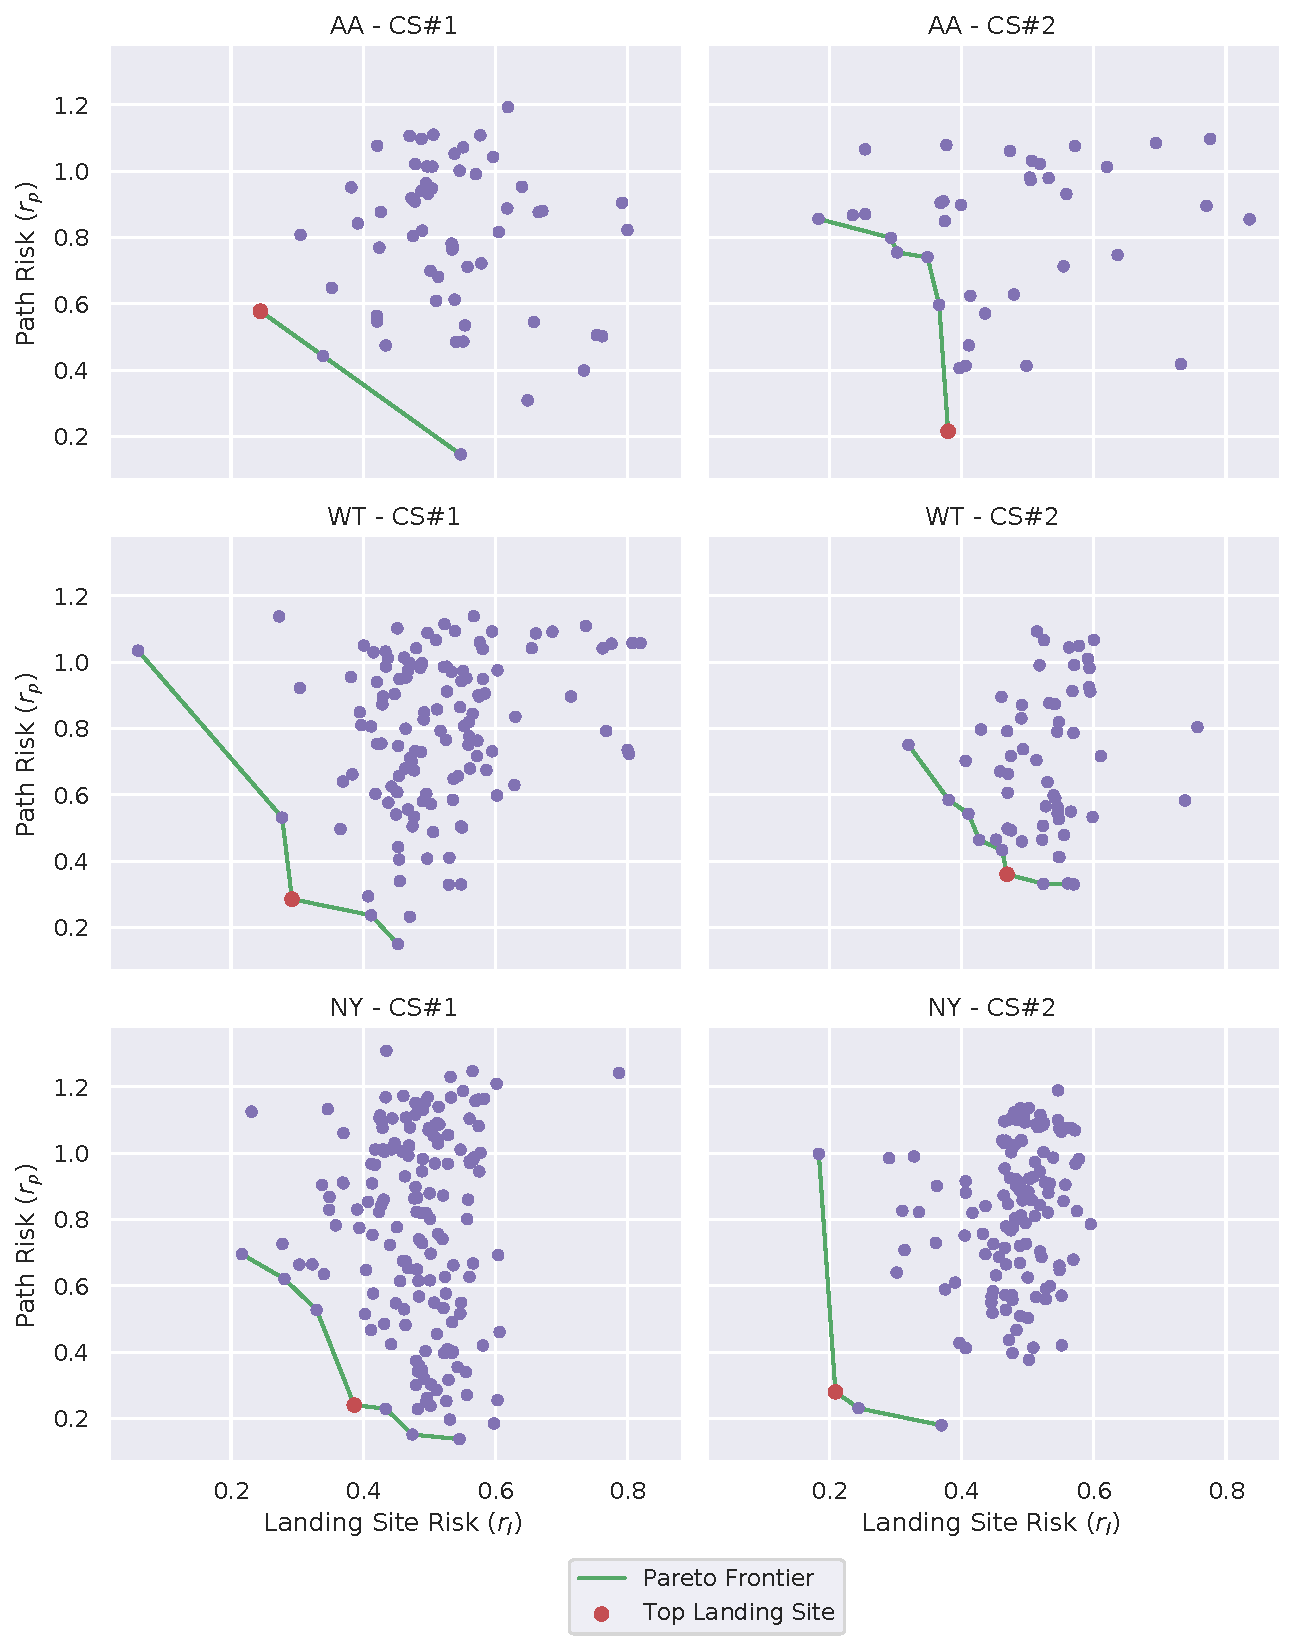
\includegraphics[clip, trim=0.2cm 0cm 0cm 0cm, width=.80\linewidth]{chapter_5_mapping/imgs/all_pareto.pdf}
    \caption[Pareto frontier of case studies]{Pareto frontier of case studies. Simulation results for six case studies performed in Ann Arbor (first row), Witten (second row), and New York City (third row). The $x$ and $y$ axes are landing site risk and path risk, respectively. Each purple dots represents a landing site and its associated path, while the red dot signifies the planner's choice which minimizes total weighted risk.}
    \label{fig:ch5_all_pareto_plots}
\end{figure}

Figure \ref{fig:ch5_all_scenarios_map}a,b shows results of our map-based planner in Ann Arbor case studies 1 and 2. In case study 1 landing sties with low landing site risk are nearby, generating the Pareto frontier seen in the first row and column in \ref{fig:ch5_all_pareto_plots}. The resulting front is approximately linear and the multi-goal planner, which favors landing site risk per Table \ref{table:ch5_weights} chooses the landing site with lowest $r_l$. Case study 2 has the unfortunate situation where the best landing sites are far away, resulting in a Pareto front that has a sharp vertical drop. This drop allows the planner to make a trade-off between landing site risk and path risk which favors the point near the bottom of the front which represents a landing site near the UAS.

Witten case studies are shown in Figure \ref{fig:ch5_all_scenarios_map}c,d.   The Pareto front for case study 1 is nearly linear with the exception of a dip caused by one landing site (red point). The significant drop in path risk causes it to have the minimum total risk and be selected. Case study 2 shows a Pareto front shifted far to the right, indicating that few landing sites with low $r_l$ are available. In addition few landing sites are immediately nearby for landing, forcing the planner to select a landing site which has a higher total risk than seen in case study 1.

New York City case studies are shown in Figure \ref{fig:ch5_all_scenarios_map}e,f. A clear difference from the prior city case studies is the increased number of landing sites that are available. In New York hundreds of flat rooftops offer viable landing site options. However it should be noted that quantity does not necessarily imply quality as many of these landing sites have high landing site risk. Case study 2 shows the fortunate situation where the \ac{UAS} failure is next to a low risk landing site causing the elbow shape Pareto front in the last row/col in Figure \ref{fig:ch5_all_pareto_plots}. This point (marked in red) is selected by our planner because it provides the minimum total risk.

% \begin{figure}[h]
%     \centering
%     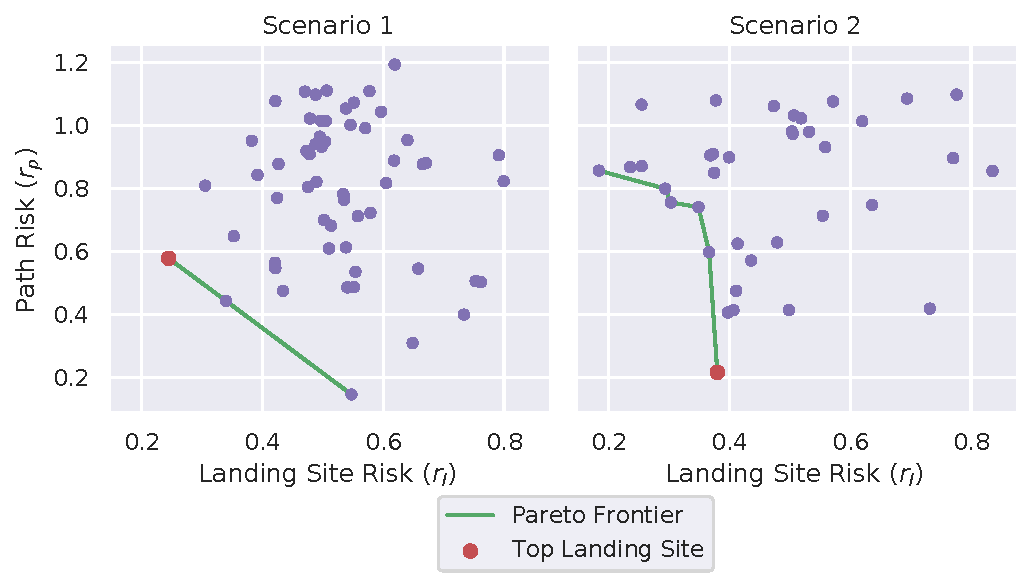
\includegraphics[clip, trim=0.2cm 0cm 0cm 0cm, width=300pt]{chapter_5_mapping/imgs/annarbor_pareto.pdf}
%     \caption{Pareto Frontier}
%     \label{fig:ch5_aa_pareto_plots}
% \end{figure}


% \begin{figure}[h]
%     \centering
%       \begin{subfigure}[b]{0.47\linewidth}
%         \centering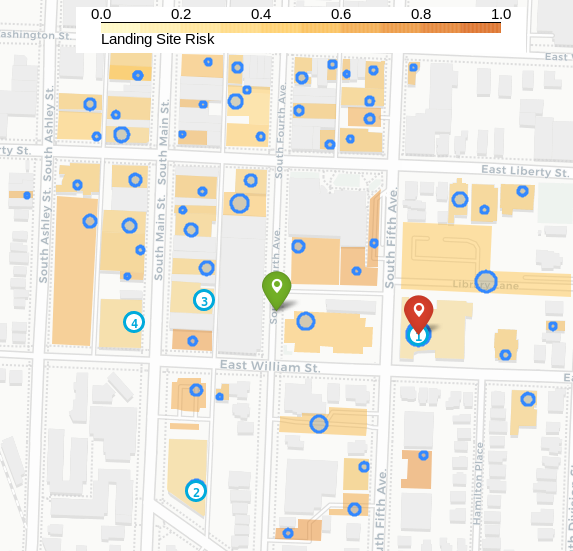
\includegraphics[clip, width=150pt, height=150pt]{chapter_5_mapping/imgs/annarbor_scenario_2.png}
%         \caption{\label{fig:ch5_aa_map1}}
%       \end{subfigure}
%       \begin{subfigure}[b]{0.47\linewidth}
%         \centering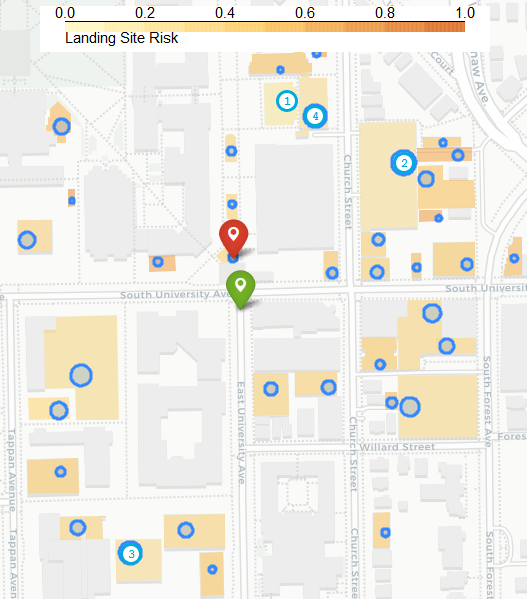
\includegraphics[width=150pt, height=150pt]{chapter_5_mapping/imgs/annarbor_scenario_4.png}
%         \caption{\label{fig:ch5_aa_map2}}
%       \end{subfigure}
%          \caption{Maps of Ann Arbor for failure Scenario 1 (a) and 2 (b).  Failure position of the \ac{UAS} is indicated by the green marker. Landing site risk is colorized from low (yellow) to high (dark orange) risk, with associated touchdown sites marked as blue circles. The lowest risk landing sites are ranked and marked with blue numbered icons. Our planners chosen landing site is marked in red which trades off between landing site and path risk. Map from \copyright OpenStreetMap contributors and \copyright CARTO.}
%      \label{fig:ch5_aa_scenarios_map}
% \end{figure}


% DONT use subfigure captions, the image is too big and wont find on the page
% Unless we somehow break it apart

% Map from \copyright OpenStreetMap contributors and \copyright CARTO.






% \begin{figure}[ht]
%   \centering
%   \begin{subfigure}[b]{0.95\linewidth}
%     \centering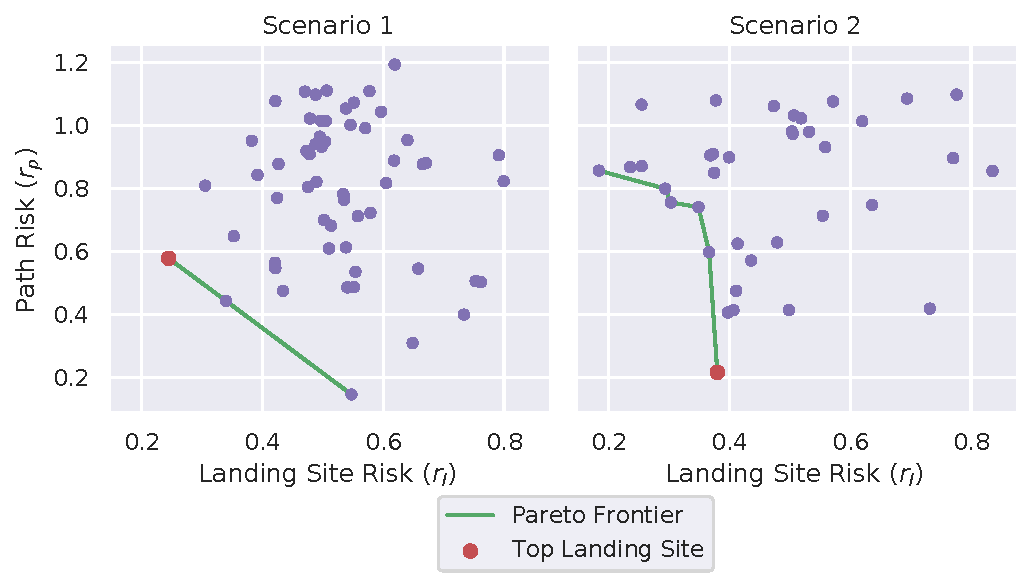
\includegraphics[clip, trim=0.2cm 0cm 0cm 0cm, width=300pt]{chapter_5_mapping/imgs/annarbor_pareto.pdf}
%     \caption{\label{fig:ch5_aa_pareto}}
%   \end{subfigure}
%   \begin{subfigure}[b]{0.47\linewidth}
%     \centering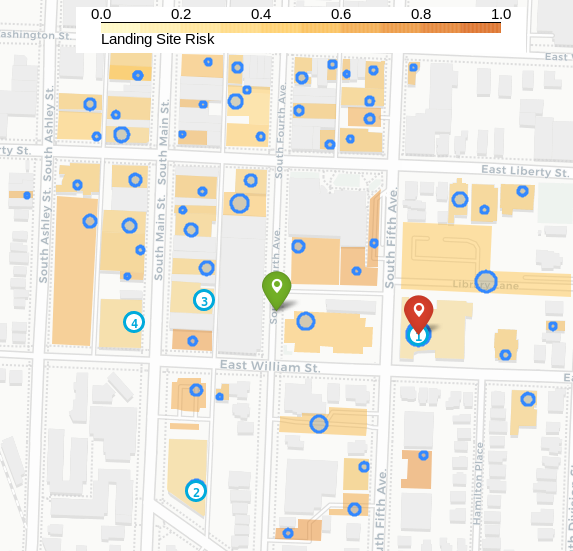
\includegraphics[clip, width=150pt, height=150pt]{chapter_5_mapping/imgs/annarbor_scenario_2.png}
%     \caption{\label{fig:ch5_aa_map1}}
%   \end{subfigure}
%   \begin{subfigure}[b]{0.47\linewidth}
%     \centering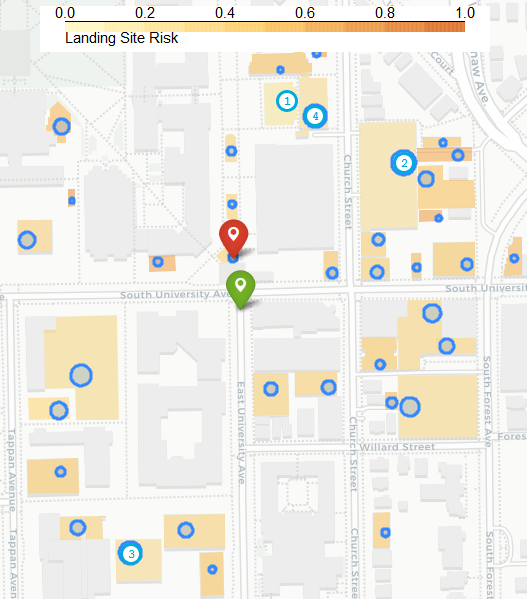
\includegraphics[width=150pt, height=150pt]{chapter_5_mapping/imgs/annarbor_scenario_4.png}
%     \caption{\label{fig:ch5_aa_map2}}
%   \end{subfigure}
%   \caption{stuff}
%   \label{fig:ch5_aa_scenarios}
% \end{figure}



\subsection{Urgent Landing Statistical Analysis}\label{sec:ch5_meta_analysis}

Two practical questions emerge from this study.  First, how practical will it be for a small \ac{UAS} to land in each analyzed city?  Second, how quickly can the \ac{UAS} identify a solution using the Algorithm 2 planner?  Section \ref{sec:ch5_footprints} analyzes the minimum search radius needed to guarantee a landing site, offering a practical constraint on required \ac{UAS} range for an urgent landing in a given region. Section \ref{sec:ch5_key_metrics} analyzes key performance metrics of our proposed planner.

\subsubsection{Minimum Radius Footprint}\label{sec:ch5_footprints}

A search radius footprint, $R$, determines the maximum distance the planner will search for available landing sites.  If this number is too small it is possible that no landing sites will be returned, potentially requiring an unsafe ditching / flight termination. It is therefore desirable to quantify the minimum radius footprint necessary to guarantee at least one landing site will be found anywhere in a mapped region.  Figure \ref{fig:ch5_farthest_landing_site} shows a planning area map of Ann Arbor, Witten, and New York in meters. All landing sites with a minimum radius of two meters are denoted by blue circles while the center of the red circle represents the point on the map farthest  from any landing site. This point is found by finding the largest inscribed circle contained in the map that does not touch or contain any landing site. These maximum distances, $d_{max}$, are computed to be 123, 106, and 207 meters for Ann Arbor, Witten, and New York, respectively. Note that this technique does not account for points near the edge of the map which may be farther from landing sites (such as northeast Manhattan).  Therefore to guarantee a landing site is found with $R \ge d_{max}$, the operating region of this city map must be shrunk by each city's respective $d_{max}$. Alternatively, one can set $R \ge 2 \cdot d_{max}$.


\begin{figure}[!t]
 \centering
 \begin{minipage}[b]{0.50\textwidth}
   \begin{subfigure}[b]{\linewidth}
    \centering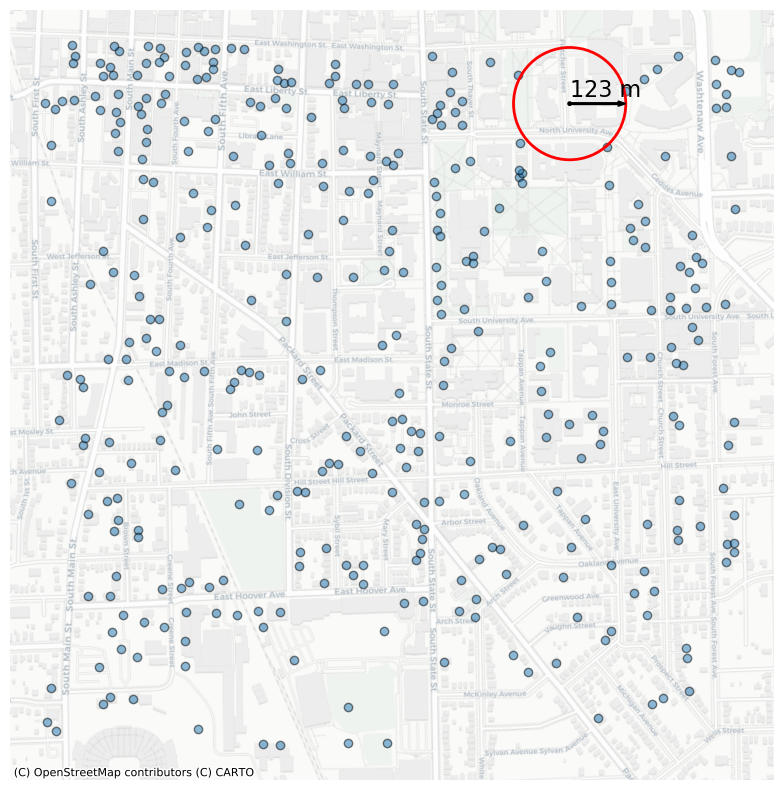
\includegraphics[clip, trim=0.0cm 0.0cm 0.0cm 0.0cm, width=\linewidth]{chapter_5_mapping/imgs/annarbor_ls_max_dist.png}
     \caption{Ann Arbor}\label{subfig-2:dummy}
   \end{subfigure}\\[\baselineskip]
   \begin{subfigure}[b]{\linewidth}
    \centering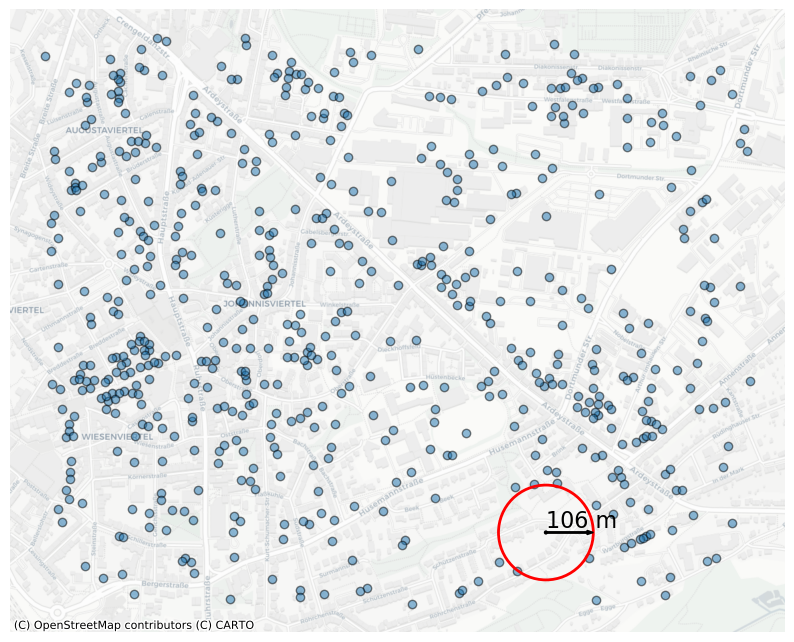
\includegraphics[clip, trim=0.0cm 0.0cm 0.0cm 0.0cm, width=\linewidth]{chapter_5_mapping/imgs/witten_ls_max_dist.png}
     \caption{Witten}\label{subfig-3:dummy}
   \end{subfigure}
 \end{minipage}
 \hfill
 \begin{subfigure}[b]{0.45\textwidth}
 \centering
 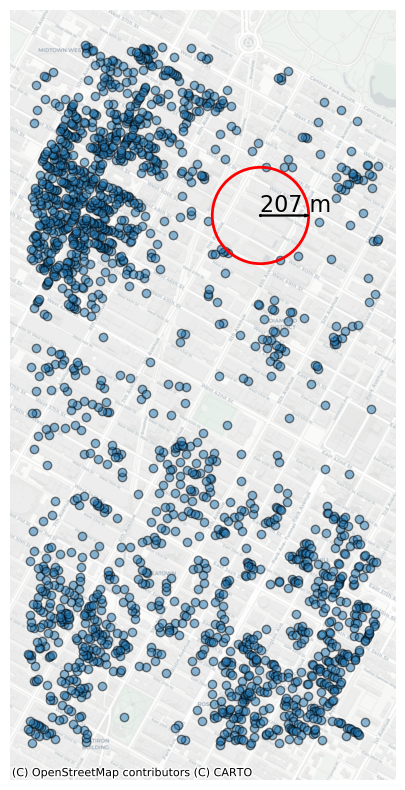
\includegraphics[clip, trim=0.0cm 0.0cm 0.0cm 0.0cm, width=\linewidth]{chapter_5_mapping/imgs/newyork_ls_max_dist.png}
%   \rule{\linewidth}{\dimexpr 2\linewidth+2\baselineskip+6pt}
   \caption{New York}\label{subfig-1:dummy}
 \end{subfigure}
 \caption[Maximum distance between landing sites]{Maximum distance between landing sites. Each landing site is displayed as a blue circle with the red circle center labelling the point farthest from any landing site. Maps from \copyright OpenStreetMap contributors and \copyright CARTO. License: Open Database License: https://www.openstreetmap.org/copyright}\label{fig:ch5_farthest_landing_site}
\end{figure}



\subsubsection{Performance Benchmarks}\label{sec:ch5_key_metrics}

Monte Carlo simulations were performed to gather four key performance metrics of our proposed urgent landing planner: number of available landing sites in the landing footprint, database query time, multi-goal planning time, and number of landing site searched ($k$ in Theorem \ref{thm:ch5_thm1}). All results were computed using a desktop computer running an AMD 3900X 4.1 GHz processor. Each city had 500 uniformly sampled failure positions for which our framework provided a landing site and path with minimum total risk. Parameters were set to those from Table \ref{table:ch5_weights}. Figure \ref{fig:ch5_random_stats} displays a swarm plot with a box and whisker plot overlay showing results. Each data point is shown with the box capturing the inter-quartile range, the line in the box representing the median, and whiskers denoting 0-95th percentile. Outliers, if existing, are labeled in the top right of the graph. 

Figure \ref{fig:ch5_random_stats}a shows the number of available landing sites in the reachable footprint for each of the cities.  Ann Arbor has the least number of landings sites, followed by Witten and then New York. Manhattan in particular has the highest number of possible landings sites.  In some sections of the borough there are more than 300 landing sites within reach; this is most often near small clustered flat buildings found in the Northeast map region per Figure \ref{fig:ch5_all_ls_risk}c. However, in one particular case there is only one landing site available in Southern Central Park. In all simulations at least one landing site is available.

Figure \ref{fig:ch5_random_stats}b displays the number of milliseconds needed to query the database to provide available landing sites $\mathcal{S}_{ls}$. The median time to execute this geospatial query is under 2 ms for all cities. New York once again has a longer tail distribution since hundreds of possible landing sites are returned. This query is made efficient through the use of R* trees for spatial indexing allowing for fast lookup in the database.

Figure \ref{fig:ch5_random_stats}c shows multi-goal planner execution time in milliseconds.  Mean planning times are 2.0, 3.1, and 9.4 milliseconds for Ann Arbor, Witten, and New York, respectively. Although the mean is low, all cities have a long tail distribution, with New York requiring up to 166 milliseconds in one scenario. Some scenarios take longer than average because the 3D octile distance heuristic underestimates true path length particularly in New York due to of its many high rise buildings presenting obstacles to be avoided. The degraded heuristic affects the planner in two ways: A* path planning takes longer due to substantial search node expansion, and the multi-goal planner must search for more landing sites to prove the risk-optimal site is found. Figure \ref{fig:ch5_random_stats}d shows the number of landing sites searched by the multi-goal planner, i.e., the number of loop iterations in Algorithm \ref{alg:ch5_multi_goal}. Each of these iterations requires an independent A* path planning procedure. The worst case is found in New York with 11 planning iterations requiring an overall multi-goal planning time of 166ms.  

% \begin{table}[h]
% \centering
% \caption{Multi Goal Planning Time}
% \label{table:ch5_planning_time}
% \begin{tabular}{@{}lccc@{}}
% \hline\noalign{\smallskip}
% City      & mean & std  & max   \\ 
% \noalign{\smallskip}\hline\noalign{\smallskip}
% Ann Arbor & 2.0  & 4.1  & 60.7  \\
% Witten    & 3.1  & 6.2  & 59.8  \\
% New York  & 9.4  & 19.6 & 165.8 \\ 
% \noalign{\smallskip}\hline\noalign{\smallskip}
% \end{tabular}
% \end{table}


\begin{figure*}[ht]
  \centering
  \begin{subfigure}[b]{0.475\textwidth}
    \centering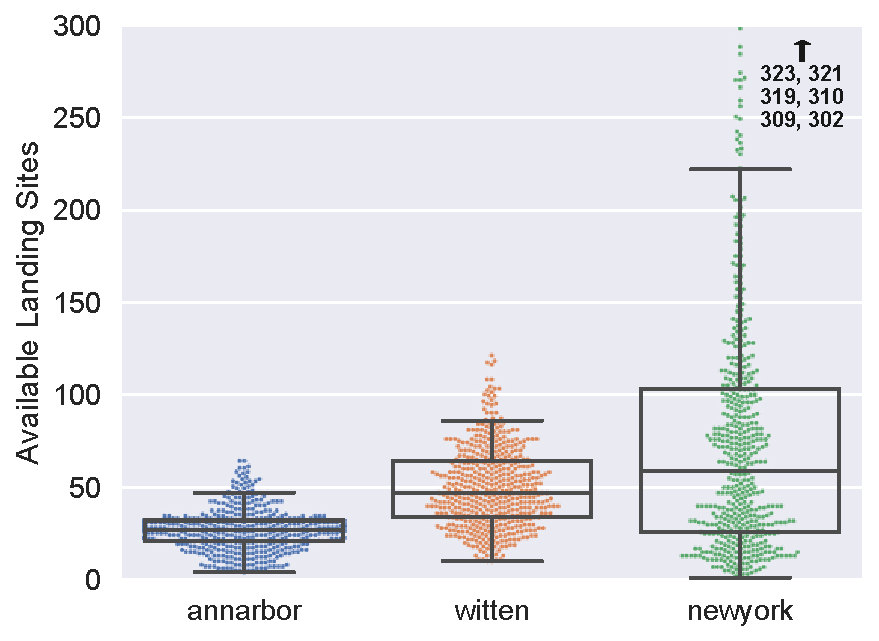
\includegraphics[width=\textwidth]{chapter_5_mapping/imgs/random_num_available_ls_bw.pdf}
    \caption{\label{fig:ch5_random_num_ls}}
  \end{subfigure}
  \hfill
  \begin{subfigure}[b]{0.475\textwidth}
    \centering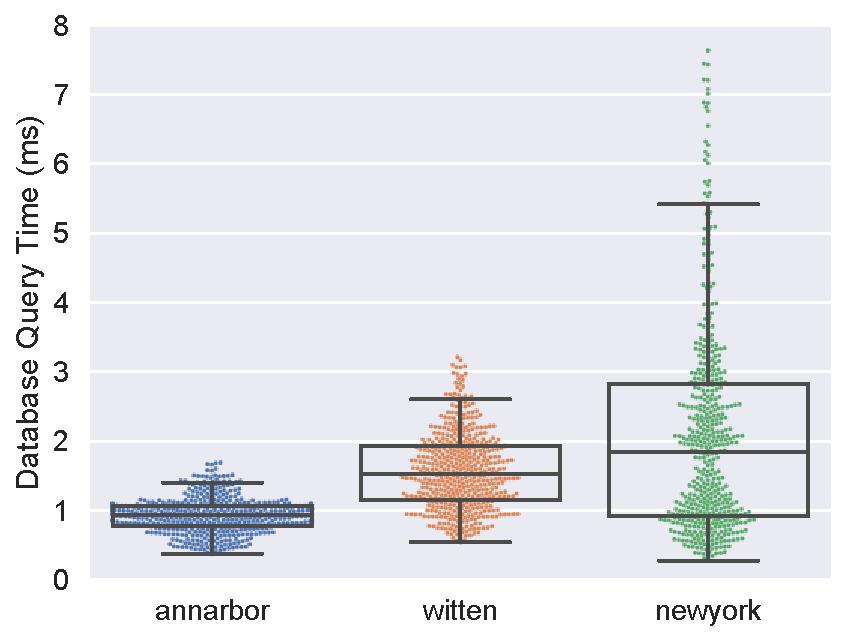
\includegraphics[width=\textwidth]{chapter_5_mapping/imgs/random_db_time_bw.pdf}
    \caption{\label{fig:ch5_random_db_time}}
  \end{subfigure}%
  \vskip\baselineskip
  \begin{subfigure}[b]{0.475\textwidth}
    \centering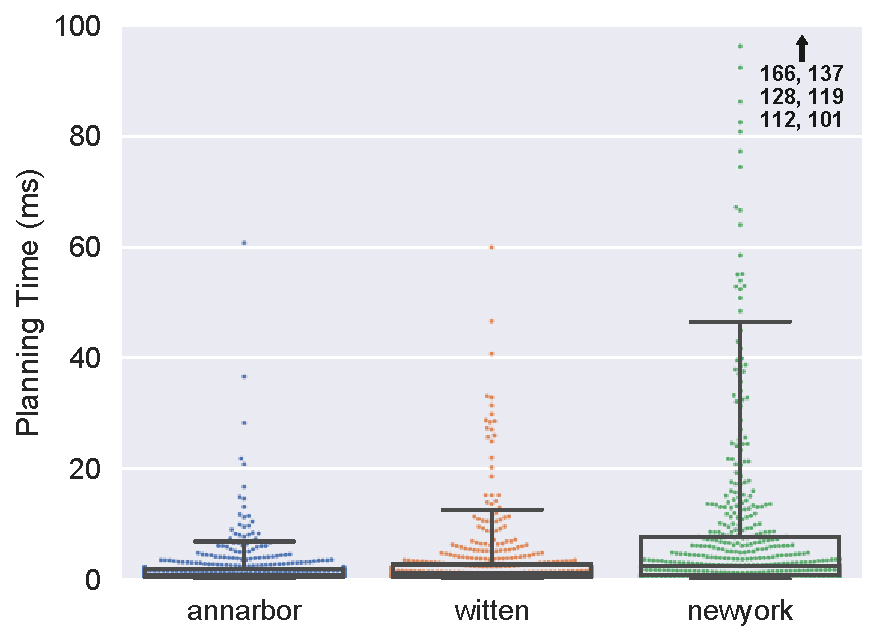
\includegraphics[width=\textwidth]{chapter_5_mapping/imgs/random_time_bw.pdf}
    \caption{\label{fig:ch5_random_plan_time}}
  \end{subfigure}%
  \quad
  \begin{subfigure}[b]{0.475\textwidth}
    \centering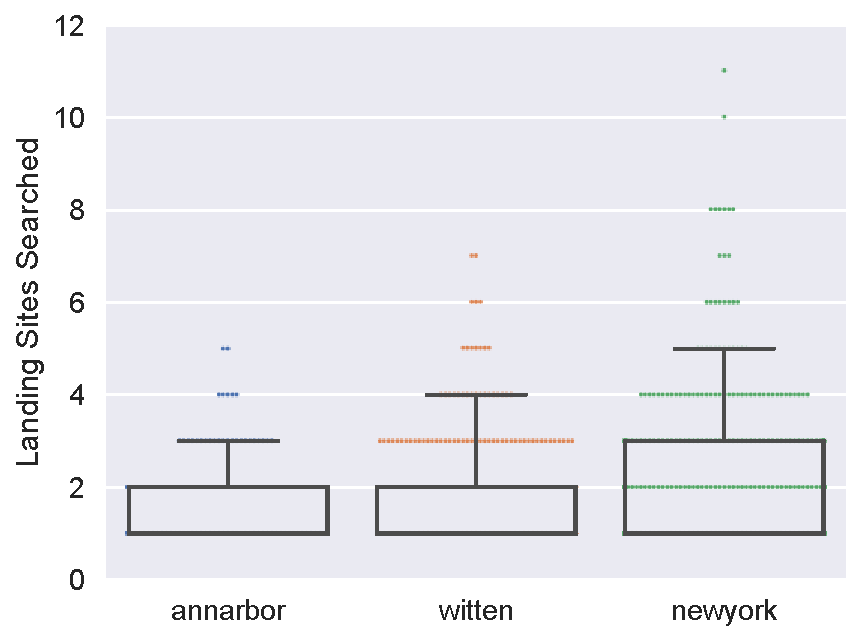
\includegraphics[width=\textwidth]{chapter_5_mapping/imgs/random_total_goal_searches_bw.pdf}
    \caption{\label{fig:ch5_random_ls_searched}}
  \end{subfigure}%
  \caption[Metrics for map-based planner]{Metrics for map-based planner. Comparison between the cities of Ann Arbor, Witten, and New York in 500 random \ac{UAS} initial positions with a search radius of 250 m. Each data point is shown with the box capturing interquartile range and whiskers denoting 0-95th percentile. Statistics are provided for number of available landing sites (a), time to query the database (b), time to find the risk-optimal landing site/path pair (c), and number of landing sites searched (d).}
  \label{fig:ch5_random_stats}
\end{figure*}


\section{Discussion and Future Work}


% Results show that buildings with flat rooftops can be found through a neural network and flat surfaces isolated with Polylidar3D.  Optimal touchdown points can be computed and used to augments existing conventional landing site databases. This   Monte Carlo simulations indicate that our proposed multi-goal planner is able to efficiently search and find a risk-optimal landing site/path pair in less than 100 ms on average in a variety of cities and failure positions. 

The presented landing site risk model evaluates risk to both the vehicle and nearby property. Vehicle risk currently includes terrain type, planarity, and area size metrics. However, future work should investigate load bearing capability of buildings, ingress and egress clearance and complexity, wind patterns, and the direction of abort paths \cite{scherer_autonomous_2012}. The risk to overflown population could not be calculated in this chapter because population density data at high spatial resolution is not widely publicly available.  Census records have low spatial resolution and do not accurately represent population distribution during the day. Anonymized call detail records can be used to augment this data to create temporal population models but are only available as sample datasets in a few regions \cite{di_donato_evaluating_2017}. Additionally, the population models must have high spatial resolution in order to discriminate between landing sites within the small radial footprints needed for sUAS urgent landing. This data will allow a more complete picture of the risk to humans especially when coupled with building sheltering factors \cite{melnyk_third-party_2014-1}.

This is unfortunate because the authors, like others \cite{ancel_real-time_2017, di_donato_evaluating_2017}, view the risk to humans as the most critical component when assessing risk. Such data will allow a more complete picture of the risk to humans when searching for landing sites in small radial footprints. 

The risk models presented in this chapter closely follow multiattribute utility theory while substituting utility maximization for risk minimization\cite{Wickens2015}. This theory assumes that the overall risk of a decision is the sum of the magnitude of each attribute multiplied by a risk score. These magnitudes are subjective and require thoughtful human determination. However, humans in urgent problem solving situations do not have time to consider all factors and often rely on simplified heuristics or shortcuts \cite{2003_technical_review_human_error}. Decisions generated with heuristics are often acceptable (satisficing), quickly determined, but non-optimal \cite{wickens_5_1988}. Results from this chapter indicate that our proposed multi-goal planner is quick, providing a risk-optimal landing site/path decision in less than 100ms. Future work should be performed to gather expert pilot opinions on whether the proposed metrics are sufficient and if additional metrics are needed. Participant will also rank, categorize, and group the most important attributes. Scenarios similar to the presented case studies can be shown where pilots will choose a landing site/path pair. A fully integrated visualization of 2D maps, 3D environments, and risk graphs can be presented to allow research participants to make informed decisions. The interface will be designed such that participants can dynamically adjust rankings and/or weights of attributes to visualize changing Pareto frontiers.

% The presented case studies demonstrate the trade-off between landing site and path risk through Pareto frontiers. Numerous risk-minimal landing sites are available in cities. However a singular site must be chosen that balances both objectives. This weighting criterion is subjective and is often the product of human value judgement. The appr



% The addition of rooftop landing sites greatly expanded the number of available landing sites. 

% Should we consider anythign but population?
% Real-time Risk Assessment Framework for Unmanned Aircraft System (UAS) Traffic Management (UTM)
% Although financial impacts ofUAS crashes can be substantial,5(e.g., \ac{UAS} replacement value, repair of damage to property, environmentalcleanup costs, etc.)  within the URAF methodology only the human safety or loss of life was considered asthe risk assessment metric



% Improvement to landing site risk
%     Need population information that is more dynamic. Static pop. information is only useful at night.
%     Need information about the materials of the landing site
%     Need information about the use of the landing site (school, busy park, open field)
%     Need information about the complexity of landing site area (ingress). E.g many obstacles, nearby power lines, etc.
  
  
% ** Evaluation Landing Site Risk ***  
% From Here: https://www.sciencedirect.com/science/article/pii/S0921889012001509#br000085
% The ground conditions that need to be considered for assessing an LZ are
%     minimum size of the site
%     skid contact
%     static stability on ground based on the center of gravity of the aircraft
%     load bearing capability of the contact surface
%     loose foreign objects (FOD) and vegetation surrounding the site
%     clearance of aircraft/rotor with surrounding terrain and objects

% while the approach conditions are the
%     clearance of the path with respect to the terrain
%     wind direction
%     direction of the abort paths.

% The ground path needs to be evaluated for traversability cost and path length.
% Additionally the algorithm also checks that an abort path that deviates by at most 45° from the approach is obstacle free. This is an added measure of safety because we can abort an approach at any time by following the abort path from the current altitude.

% ** End ***

% Propose work where landing sites and case studies are presented to experience pilots. Design questionaries (debriefing forms) about what landing sites are best.


% Accident investigations and empirical studies suggest that high stress levels cantrigger attentional narrowing

% % The Effects of High Stress on Attention: A First Step Toward Triggering Attentional Narrowing in Controlled Environments 
% % not only did participants detect fewer deviations, but it took them longer to correctthe deviations and their responses were less accurate.

% Challenging the assumptions that distance and risk of a landing site are the primary factors when determining an optimal path. 
% Weather - Weather:  As noted in the National Transportation Safety Board (NTSB) aviation accident database [40], adverse weather conditions (e.g., wind, visibility/ceiling, turbulence, up/downdraft, wind shear, thermal lift, icing, lighting, etc.) accounted for approximately 20\% of total aircraft accidents from 2003 through 2007. But does weater play a factor in such localized areas and conditions?
% Ingress and Egress Paths

% Discuss Human factor stuff here

% Future Work on Rooftops for sheltering rates:
% The Range Safety Group28proposed employing the building classes givenin Table 6 for their vulnerability models.  The vulnerability models define the relationship between object(e.g., UAS) mass, ballistic coefficient, and the effective casualty area.  Figure 5 provides the model used fora class B roof.  A more detailed discussion regarding the development and use of the vulnerability modelscan be found in the FAA Flight Safety Analysis Handbook34and in Safety Design for Operations.35



\section{Conclusion}\label{sec:ch5_conclusion}

\ac{UAS} operating in cities need to identify safe landing sites and associated paths in real-time whenever an urgent landing is required. This chapter proposed the use of nearby flat rooftops to augment traditional emergency landing sites such as parks and fields. We showed that fusion of deep learning for roof shape identification and computation geometry for flat surface extraction results in suitable landing site identification.  Landing site locations and associated risks were stored onboard \ac{UAS} along with obstacle and risk maps of the local flight area.
While previous risk-based planners have been proposed, our map-based planner is the first to explicitly trade off landing site risk and path risk to minimize combined total risk. Our multi-goal planning algorithm efficiently selected the landing site/path pair guaranteed to minimize a weighted total risk function. Landing site databases and 3D risk maps were generated for three diverse cities with results presented from six case studies. Additional Monte Carlo simulations were run on all three cities to assess key performance metrics, showing that our planner finds risk-optimal landing sites and paths in less than 50ms for 95\% cases. Worst-case execution time across our tests was 166ms in New York City. Future work can address this with a distributed or cloud-based path planner that offers speed up through parallelization. Additional risk factors such as wind patterns, rooftop material and strength, and dynamic population data will improve results. Ultimately, multiple \ac{UAS} sensor data streams can be incorporated into mapping and real-time planning systems to refine risk databases.